%!TEX TS-program = xelatex
%!TEX encoding = UTF-8 Unicode

\documentclass{Dissertate}

%!TEX root = thesis.tex

% EXAMPLE CHAPTHER 

\newglossaryentry{word}{
	name={This is a word},
	description={This is how a glossary word seems.
%		\cite{source}
	}
}

%INTRODUCTION

\newglossaryentry{Broadband networking}{
	name={Broadband networking},
	description={In general, broadband refers to telecommunication in which a wide band of frequencies is available to transmit information. Because a wide band of frequencies is available, information can be multiplexed and sent on many different frequencies or channels within the band concurrently, allowing more information to be transmitted in a given amount of time (much as more lanes on a highway allow more cars to travel on it at the same time)
	\cite{broadband}}
}

\newglossaryentry{Low latency}{
	name={Low Latency Communication},
	description={Low latency describes a computer network optimized to process a very high volume of data messages with minimal delay (latency). These networks are designed to support operations that require near real-time access to rapidly changing data
	\cite{low_latency}}
}

\newglossaryentry{Core network}{
	name={Core Network},
	description={The core network of a telecommunication infrastructure represents the services that interconnect the main components that create the backbone, which are usually routers and switches}
}

\newglossaryentry{LTE}{
	name={Long-Term Evolution (LTE)},
	description={Long-Term Evolution is a standard for wireless broadband communication for mobile devices and data terminals}
}

%CHAPTER 2

\newglossaryentry{Roadmap}{
	name={Roadmap},
	description={A roadmap is a strategic plan that defines a goal or desired outcome and includes the major steps or milestones needed to reach it}
}

\newglossaryentry{Repository}{
	name={Repository},
	description={A software repository is a storage location from which software packages, verisoned and well documented, may be retrieved and installed on a computer}
}

\newglossaryentry{Milestone}{
	name={Milestone},
	description={A milestone is a specific point in time within a project lifecycle used to measure the progress of a project toward its ultimate goal.
	Milestones are associated with working deliverables that, in case of future flops, can be used as checkpoints}
}

%CHAPTER 3

\newglossaryentry{Framework}{
	name={Framework},
	description={
		A framework is an abstraction that establishes common practives for creating, interpreting, analyzing and using architecture descriptions within a particular domain of application}
}

%CHAPTER 5

\newglossaryentry{CentOS}{
	name={CentOS},
	description={CentOS is an Enterprise Linux distribution based on the sources from Red Hat Enterprise Linux}
}

\newglossaryentry{Virtual Machine}{
	name={Virtual Machine},
	description={A Virtual Machine (VM) is an emulation of a computer system}
}

\newglossaryentry{Remmina}{
	name={Remmina},
	description={Remmina is a is free and open-source remote desktop client for Linux and other Unix-like systems that allows connecting with other systems from terminal or graphical interfaces}
}

\newglossaryentry{H2 database}{
	name={H2 database},
	description={H2 is an open-source lightweight Java database. It can be embedded in Java applications or run in the client-server mode}
}

\newglossaryentry{Cookie}{
	name={Cookie},
	description={A cookie is a text file that a Web browser stores on a user’s machine. Cookies are a way for Web applications to maintain application state. They are used by websites for authentication, storing website information/preferences, other browsing information and anything else that can help the Web browser while accessing Web servers\cite{cookie}}
}

\newglossaryentry{Context Path}{
	name={Context Path},
	description={The context path is the prefix of a URL path that is used to select the context(s) to which an incoming request is passed\cite{configuring-contexts}}
}

\newglossaryentry{VPN}{
	name={Virtual Private Network (VPN)},
	description={A Virtual Private Network extends a private network across a public network, and enables users to send and receive data across shared or public networks as if their computing devices were directly connected to the private network}
}


%CCONCLUSIONS

\newglossaryentry{Container}{
	name={Container},
	description={A Docker container is an open source software development platform. Its main benefit is to package applications in containers, allowing them to be portable to any system running a Linux or Windows operating system (OS)\cite{docker}}
}



\makeglossaries

%!TEX root = thesis.tex

\begin{document}
		
	\raggedbottom

	%!TEX root = ../thesis.tex
% Some details about the dissertation.

\title{Open LoRa mesh network for\\IoT-based air quality sensing}

\author{Voinea Stefan Ciprian}
 
%If you have one advisor
\advisor{Claudio Enrico Palazzi}

%If you are coadvised
%\coadvisorOne{Pietro Manzoni}
\coadvisorOne{~}
\coadvisorOneUniversity{Second advisor's University}

\mastername{Computer Science}

% School name and location
\university{University of Padova}
\universitycity{Padova}
\universitystate{Italy}

\definecolor{SchoolColor}{rgb}{0.71, 0, 0.106} % UNIPD red
\definecolor{chaptergrey}{rgb}{0.61, 0, 0.09} % dialed back a little
\definecolor{midgrey}{rgb}{0.4, 0.4, 0.4}




	% \maketitle
	% \copyrightpage

	\frontmatter
	
	\setstretch{\dnormalspacing}
	
	% Include chapters
	\setcounter{chapter}{0} 		% Start chapter numbering at 1
	% %!TEX root = ../thesis.tex

\begin{savequote}[75mm]
This is a quote
\qauthor{This is the author of the quote}
\end{savequote}

\chapter{This is a chapter}\label{ch:chapter_reference}

	\lipsum[1-2]
	
	\newpage
	
	\section{Section one}\label{sec:section_one_reference}
	
		Let me list some useful commands:
		\begin{itemize}
			\item This is a \Quote{quote}.
			\item This, \Chapref{chapter_reference}, is a chapter reference.
			\item This adds the following \gls{word}\glsadd{word} to the glossary.
		\end{itemize}
		
	%	This is a figure:	
	%	\begin{figure}[H]
	%		\centering
	%		\includegraphics[width=1\textwidth]{resources/legacy-code}\\
	%		\caption{Dilbert on legacy system infrastructures}
	%	\end{figure}
	
	\section{Section two}\label{sec:section_two_reference}
	
	\section{Section three}\label{sec:section_three_reference}
	%!TEX root = ../thesis.tex

%\begin{savequote}[75mm]
%	It always seems impossible until it's done.
%	\qauthor{Nelson Mandela}
%\end{savequote}

\chapter{Introduction}\label{chapter:introduction}

	% https://lucaspolo.eu/isaac-asimov-predicting-todays-internet-1988/
	% https://aminotes.tumblr.com/post/4994624354/isaac-asimov-predicted-the-internet-of-today-20
	
	In an interview from 1988 about school education and its relationship with the Internet, Isaac Asimov, one of the 20th century's most prolific science fiction writers, said ``\textit{now, with the computer, it's possible to have a one-to-one relationship for the many. Everyone can have a teacher in the form of access to the gathered knowledge of the human species}''.
	
	At the time of writing, many things have changed since that interview: people now live in an \textit{hyperconnected world}, where accessing Internet is considered a right, so that everyone has the same learning opportunities.
	
	According to Cisco's 2018 - 2023 Internet Report, ``the number of devices connected to IP networks will be more than three times the global population by 2023'' \cite{cisco1}.
	Authors also predict there will be 29.3 billion networked devices by 2023, a major increase from 18.4 billion in 2018. 
	% https://www.cisco.com/c/en/us/solutions/executive-perspectives/annual-internet-report/air-highlights.html
	Of al these, 50\% is represented by Internet of Things, or IoT, devices.
	
	As stated in one of Forbes's insights, ``\textit{IoT is ranked as the most important technology initiative by senior executives; more important than artificial intelligence and robotics, among many others}'', while, from an economical point of view, ``\textit{of all emerging technologies, the Internet of Things (IoT) is projected to have the greatest impact on the global economy}'' \cite{forbes}.
	The number of devices that are being connected to the Internet is growing day by day and the industry is at its highest peeks.
	
	This new paradigm of Computer Science can be considered an enabler for the sciences that need large amount of data for creating algorithms and offering better services and more well tailored products.
	The ubiquity of mobile technology has opened the door to a new era of mobile sensing. 
	
%	Starting from the Middle Ages, through the Industrial Revolutions and arriving to the Modern Era, water and air pollution have haunted people all around the world.
%	From early on, in Europe, unsanitary urban conditions favoured the outbreak of population-decimating epidemics of disease, from plague to cholera and typhoid fever.
%	% https://www.history.com/news/the-killer-fog-that-blanketed-london-60-years-ago
%	Later, with the advent of the steam engine in between of the 18th and 19th century, pollutants from factories started to spread in the air, causing problems such as smog and, in some cases, even acid rain, like the ``London Fog'' \cite{fog} in 1952.
	
	Using the data gathered until the second half of the $20^{th}$ century, computer simulations showed how the rise in CO2 levels that can lead to climate change and cause global temperatures to rise steadily in the years.
	Scientists started to take a more common approach to pollutants and climate change by developing instruments capable of more accurate readings and by better understanding how to analyze the gathered data.
	In the preface of 1981's ``\textit{The Design of Air Quality Monitoring Networks}'', the author states that ``\textit{the number of publications in the environmental area is increasing exponentially}'' \cite{airqualitynetworks}.
	This leaves one to think about the state of this research area up to date.
	
%	From the point of view of Computer Science, technology has also evolved exponentially, confirming the validity of Moore's law and increasing the accuracy of sensors and other analog peripherals used to gather data from the environment.
%	In combination with the fact that computers have also become smaller, portable and personal, a new paradigm of digital devices has emerged: the Internet of Things.

	Many publications have been studying the development of low-cost devices, focused on analyzing the quality of the surroundings of individual. 
	
	This thesis takes a focus on a particular project, MegaSense, a personal air quality device developed by the University of Helsinki.
	
	In this thesis, the architecture for connecting such devices is expanded with the use of a LoRa mesh network.
	
	\section{Contributions}\label{sec:contributions}
	
		The contributions that the work described in this thesis are
		
		% TODO explain briefly explain what are the results that have been achieved
	
	\section{Document outline}\label{sec:document_outline}
		
		This document follows an hourglass structure by first explaining in general the necessary notions to understand the work done and then going more in detail.
		The content is organized as such in the following chapters:
		% TODO create links in the document
		\begin{enumerate}
			% \setcounter{enumi}{1}			
			\item \hyperref[chapter:introduction]{\textit{Introduction}}: this introductory chapter;
			\item \hyperref[chapter:background]{\textit{Background}:}
			\item \hyperref[chapter:technologies]{\textit{Technologies}}:
			\item \hyperref[chapter:related_work]{\textit{Related work}}:
			\item \hyperref[chapter:proposed_solution]{\textit{Proposed solution}:}
			\item \hyperref[chapter:results]{\textit{Results and experimentation}:}
			\item \hyperref[chapter:conclusions]{\textit{Conclusions}}:
			
		\end{enumerate} 	% Introduction
	%!TEX root = ../thesis.tex

\chapter{Background}\label{chap:background}

	% TODO cambiare in maniera da vendere la mesh, non megasense
	This chapter introduces the background concepts necessary to understand the project presented in this thesis and why it has been developed.
	
	It first explains what the Internet of Things is, afterwards, it describes the problem with air pollution, to conclude with an overview on the background work and state or art of IoT devices capable of detecting such pollution.
	In particular, it concentrates on MegaSense, the IoT air quality sensing project which the work on this thesis builds upon.

	A deeper understanding of the related work on mesh networks can be found in chapter \ref{chapter:related_work}, where previously made projects which use a similar architecture are described.

\section{Internet of Things}

	IoT, which stands for Internet of Things, has a longer history than many people think about.
	%https//www.smithsonianmag.com/innovation/kevin-ashton-describes-the-internet-of-things-180953749/
	%http://www.itrco.jp/libraries/RFIDjournal-That%20Internet%20of%20Things%20Thing.pdf
	%https://www.rfidjournal.com/that-internet-of-things-thing
	It's name, which is now know all around the globe, has been attributed to \textit{Kevin Ashton}, who used it in a presentation about radio frequency identification (RFID) technology, at \textit{Protector \& Gamble}, in 1999 \cite{iot_definition} to describe the network connecting objects in the physical world to the Internet.
	
	This constantly expanding branch of Computer Science aims to turn physical objects, as small as they may be, into nodes of an interconnected system which opens the door to new interfaces between humans and machines and how these see the physical world.
	Its importance heavily relies on data gathered from these devices, since, in combination with other paradigms such as machine learning and Artificial Intelligence, this can be transformed into valuable information.
	The creation of models from all these inputs has given a more efficient workflow in companies and has improved certain aspects of everyday life, with wearable technologies used to enhance quality of life.
	
	% TODO inserire una frase per dire che prima di introdurre l'argomento principale ecco un paio di esempi di tecnologia IoT
	
	\subsection{Universal Product Code and Barcode}

		% https://www.thoughtco.com/bar-codes-history-1991329
		One of the first technologies that can be considered part of the IoT family, is the ``\textit{Universal Product Code}'', or \textit{UPC}.
		% todo cambiare / modificare
		It's first iteration is detailed in the patent issued to inventors Joseph Woodland and Bernard Silver on October 7, 1952, and can be described as a ``bull's eye'' symbol, made up of a series of concentric circles \cite{upc_patent}, as can be seen in Figure~\ref{fig:upc_patent}.
		
		Authors of the patent, state  that ``one application of the invention is in the so called 'super-market' field'', indicating that they already successfully identified a need to speed up and automatizing the process of paying at super-markets.
		
		\begin{figure}[h!]
			\centering
			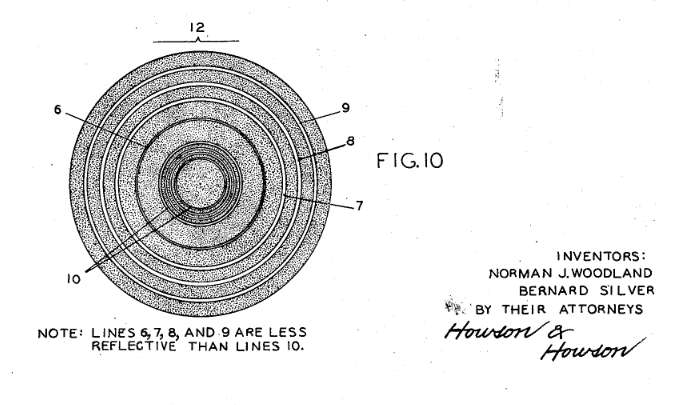
\includegraphics[width=\textwidth-4cm]{resources/img/upc_1}
			\caption{Diagrammatic view of the Universal Product Code}
			\label{fig:upc_patent}
		\end{figure}
		
		Due to the large size and low reliability of the equipment necessary to read the figure, this concept has not been immediately released for everyday use.
		Commercial adoption relied on the emergence of laser optics, which started to offer a more compact reading technology.
		
		Although, printers used to generate barcodes were vulnerable to smudge the design coped with errors as ink bleeding would result in taller bars.
		

		Only later, in 

		The first widespread 
	
		The barcode, as it is now known, was first used commercially in 1966, and it was soon realized that it would become an industry standard.
		
		The first appearance of the Universal Product Code (UPC) to the public and has become widespread, is the one developed in 1971 by George Laurer at IBM \cite{upc_ibm}.
		% TODO cambiare
		
		% TODO cambiare
		This invention offered the first way to track products and address them.
		


	% TODO cambiare titolo
	\subsection{CMU's coke machine and modern vending machines}

	%https://www.engineersrule.com/how-a-coke-machine-and-the-industrial-internet-of-things-can-give-birth-to-a-planetary-computer/
	%https://www.ibm.com/blogs/industries/little-known-story-first-iot-device/
	%https://www.cs.cmu.edu/~coke/history_long.txt

		It may come as a surprise, but connecting everyday ``things'' started around the 1980s.
		
		\noindent
		\begin{minipage}{0.5\textwidth}% adapt widths of minipages to your needs
			\centering
			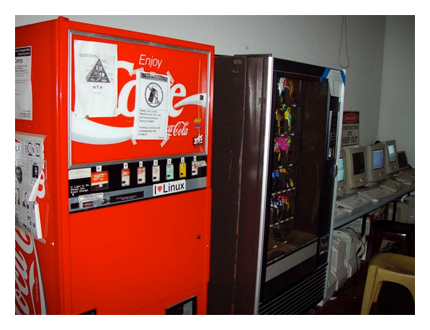
\includegraphics[width=\textwidth]{resources/img/coke}
			% \captionof{figure}{Carnegie Mellon University's ``coke machine''}
			\captionof{figure}{CMU's ``coke machine''}
		\end{minipage}%
		\hfill%
		\begin{minipage}{0.5\textwidth}\raggedright
			One of the most famous and most quoted as the first IoT device, is the Carnegie Mellon University (CMU) coke machine at the Computer Science Department.

			Communication from and to the machine, which allowed remote access, took place via Arpanet at CMU as the system predated the Internet.
		\end{minipage}
		\newline
		
		Various sensors were used to detect whether shelves were empty and to track status of coke bottles (warm, cold, empty).
		
		As expained in the official website\footnote{\url{https://www.cs.cmu.edu/~coke/history_long.txt}} dedicated to this device by the University, there are ``micro-switches in the Coke machine to sense how many bottles were present in each of its six columns of bottles''.
	
		Modern day vending machines are usually require continuous connectivity to the manufacturer's systems.
		This is not always achievable via a WiFi connection where the machines are placed, so other solutions, such as cellular connectivity, are used.
		Connection reliability in vending machines and other kiosks is important since these provide goods that can be payed by credit card, which need to establish a secure connection.
		
		They contain multiple small, but complex, systems that interact with each other, thus it is implied that this kind of machines must have installed a secure software and that they need to be as hard as possible to be tampered with, either by brute force or by software bugs.
			
		Otherwise it's not only possible that someone steals a snack or a pack of cigarettes, but some remote script may turn these machines into a botnet capable of bringing down the connectivity of an entire campus.
		Such attack has been described in Verizon's ``Data Breach Digest'' risk report from 2017, where the author states that ``the firewall analysis identified over 5,000 discrete systems making hundreds of DNS lookups every 15 minutes'' \cite{DataBreachDigest}.
		
		While credit card skimmers and chip EMV card cloners remain viable risks to the end consumer, security measures to the environment where the machines are placed must not remain an afterthought, especially when these are placed alongside other connected devices and not in their own separated network.

		% TODO completare
		% Such kind of smart vending machines have helped bring a step closer cities to become smart cities, where these can be used as a mean to place devices such as routers or public wifi access points.


	\subsection{Trends, forecasts and research directions}

		IoT and related technologies have grown exponentially since the times of CMU's coke machine.
		% TODO controllare numeri
		According to data from Microsoft Academic\footnote{\url{https://academic.microsoft.com/topic/81860439/}}, publications about the ``Internet of Things'' are growing exponentially: from the 26 in the year 2000, to 534 in 2010, 4959 in 2015, to 22454 papers published in 2020.
		This shows how much interest IoT has gathered among the scientific community. Nonetheless,
		% TODO cambiare perchè copiata totalmente
		IoT techniques still remain immature and many technical hurdles need to be overcome.

		Research directions in this new area are immense, since every physical device now represents a possible ``thing'' connected in the network and that can be interacted with and provide data.
		% TODO introdurre meglio il paper
		Authors of \cite{9319033} have highlighted ten particular topic areas that span across three layers of IoT architecture: Application, Data and Physical, as represented in Figure~\ref{iot_research_areas}.
	
		% TODO sostituire immagine con un elenco puntato?
		\begin{figure}[H]
			\centering
			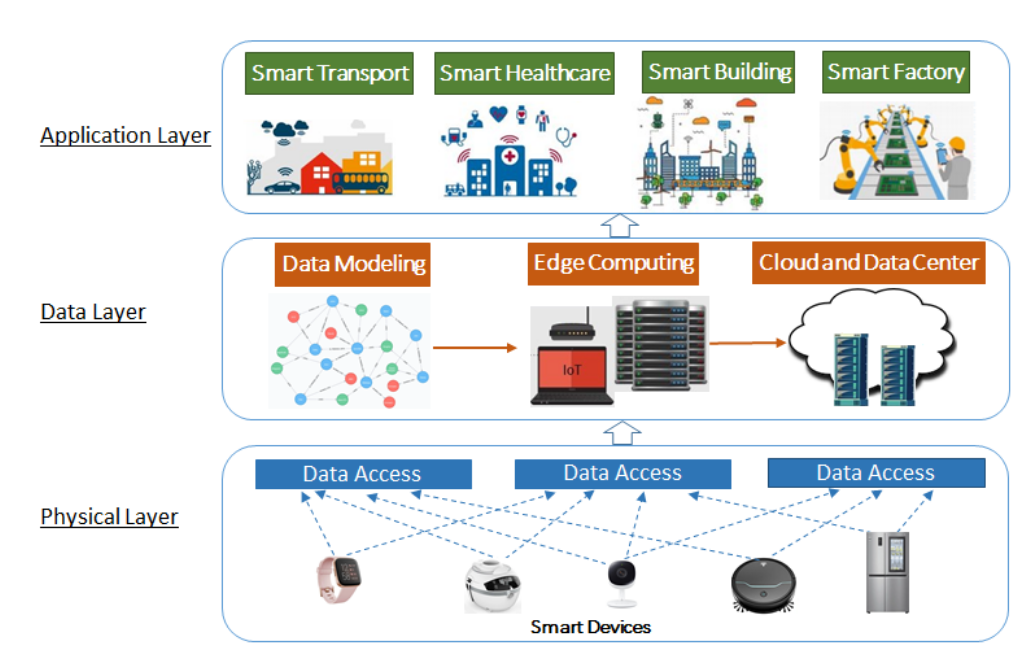
\includegraphics[width=0.8\textwidth]{resources/img/iot_research_areas}\\
			\caption{IoT research areas according to authors of \cite{9319033}}
			\label{iot_research_areas}
		\end{figure}
	
		% TODO modificare?
		These topics include ``Data-driven IoT'', ``Security, Privacy, and Trust in IoT'', ``Social IoT'', and ``Edge Computing and IoT'', which have brought the need for new paradigms of computation.
		
		Data can be created and collected at a very high speed when considering the number of devices connected.
		This has been stimulating the creation of faster and more reliable DBMSs and brokers that allow higher processing speeds and querying frequencies.
		Specialized versions of these are emerging, each fitted for different scenarios, that may range from a fully online (or as a service with products such as AWS IoT Core\footnote{\url{https://aws.amazon.com/iot-core/features/}}) infrastructure to fully on premise one.
		% TODO fare esempi?
		
		Another important aspect is the architecture of the network, which needs to take in consideration the aspects such as heterogeneity of the devices connected, velocity of data that flows across and scalability.
		Thus, paradigms like Cloud Computing, Fog Computing and Edge Computing have emerged.
		
		% TODO rifare immagine
		\begin{figure}[H]
			\centering
			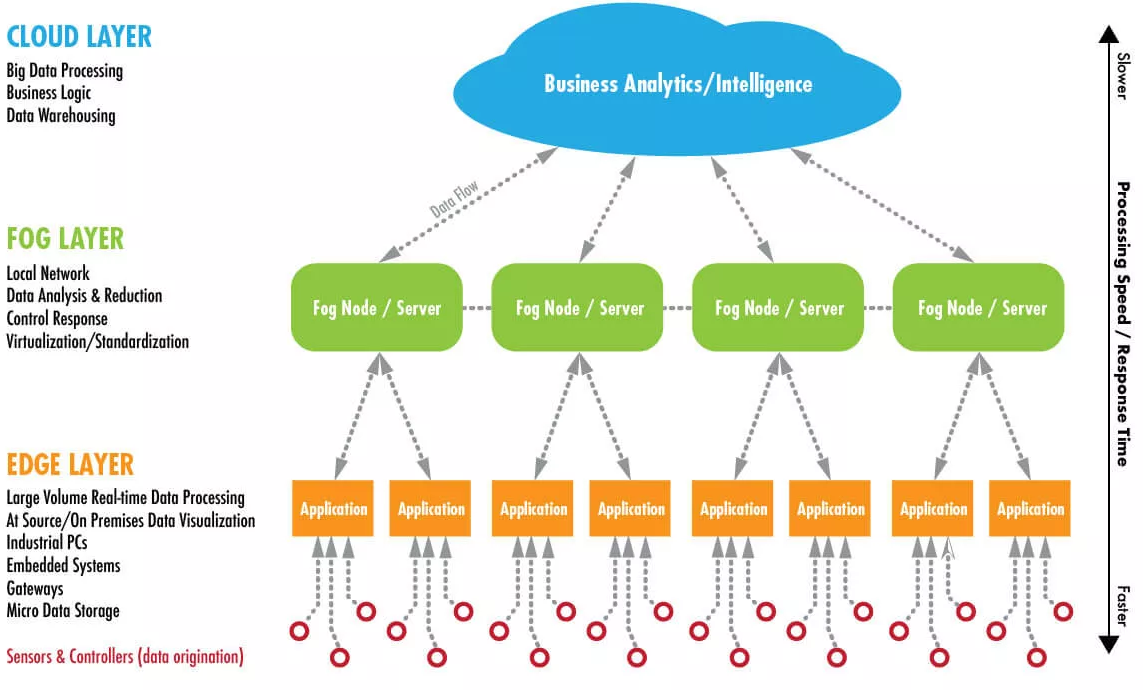
\includegraphics[width=0.75\textwidth]{resources/img/computing_paradigms.png}\\
			\caption{Edge, Fog and Cloud Computing}
			\label{computing_paradigms}
		\end{figure}
	
		% TODO spiegare meglio
		Each of these, places the computation on a different layer of the network, from Cloud Computing that lift off all the need for devices to compute data, to Edge Computing, where there might be specialized servers physically placed in strategic points so that they are closer to the end devices (lower latency), which may even have the ability to compute data by themselves.
		%https://www.cisco.com/c/en/us/solutions/computing/what-is-edge-computing.html
		On the other hand, Fog Computing is less aggressive than Edge Computing, and does not require the same amount of services placed near the clients, but they can be sorted among the backbone of the network.
		
		These communications do not take place only via WiFi or Ethernet.
		Given that ``things'' can be everywhere, the need for a network that can adapt to a fast paced environment is becoming a must.
		Here is where the 5th generation of cellular connectivity comes into play.
		
		%https://www.gsma.com/iot/resources/iot-5g-ltem-nbiot-opportunities-benefits/
		As described in a 2019 whitepaper by GSMA on the IoT and the use of 5G, a ``combination of 5G and wireless edge technologies will support demanding  use cases, such as autonomous driving, time-critical industrial IoT manufacturing processes and  augmented and virtual reality (AR/VR)''\cite{IoT_5g_era}.
		Compared to what is possible with other transmission technologies, 5G supports a massive number in connections, with very little latency.
			
		All of this is not only interesting from a research point of view, but also from a market point of view, where new devices, for consumer and industrial purposes, are created to suit every possible need, that is why IoT can be considered as the ``next chapter of digital communication''.
		
		% TODO riscrivere parlando di health e home automation
		The most notable example from a consumer's point of view, is the smartwatch, which started with the infamous Pebble watch, and is now considered almost a ``must-have'' extension of the smartphone.
		Not only it can be used for recreational purposes, but it is crossing the line to become medical devices, given the improving accuracy with which they record data.
		Data that, in conjunction with AI, can be used to predict heart attacks \cite{7946780} or other diseases, like Hyperkalemia \cite{HYPERKALEMIA}.
		Even now IoT devices and frameworks can be used for contact tracing in order to prevent the spread of Covid-19 \cite{9181512}.
		% Although, it is important to notice that not all projects have succeed, smart glasses by google
		
%		Home automation is another big market
%		Consumers want remote control
%		of devices such as coffee pots so that they may wake up to freshly
%		brewed coffee, or cause coffee to be prepared at a precise time after
%		the completion of dinner preparations.
%		\footnote{\textit{Hyper Text Coffee Pot Control Protocol}: \url{https://datatracker.ietf.org/doc/html/rfc2324}}
		
		On the other hand, from an industrial point of view, there are 
		
		
		with Industry 4.0 and Industrial IoT (IIoT)
		
		% https://www.mdpi.com/1999-5903/12/3/46
		The growing popularity of IoT use cases in domains that rely on connectivity spanning large areas and the ability to handle a massive number of connections is driving the demand for LPWAN access technologies. 
		
%		\vspace{3cm}
%		
%		The goal of fifth-generation (5G) wireless networks and beyond is to realize connecting “anything, anyone, anytime, anywhere” [1] reliably and energy-efficiently [ M. Agiwal, A. Roy and N. Saxena, "Next generation 5G wireless networks: A comprehensive survey", IEEE Communications Surveys \& Tutorials, vol. 18, no. 3, pp. 1617-1655, 2016.]
%		
%		The more data available, the more there are opportunities for science, services, business etc. to understand and grow.
%		
%		IoT is an enabler for the sciences that need large amount of data for creating algorithms and offering better services and more well tailored products.
%		% https://www.siemens-advanta.com/blog/what-are-expected-iot-trends-2021
%		
%		Another important definition of IoT is IIoT, which stands for Industri 4.0 IoT.
%		
%		Given the importance of this economic sector, many companies, both technical and not, have analyzed the trends and have been producing forecasts about the growth of IoT.
%		% measure commercial adoption of the then-emerging technology. 
%		
%		One analysis, made by The Economist's Intelligence Unit, and sponsored by Arm \footnote{\url{https://www.arm.com/}}, states that ``More than two-thirds of respondents agree that understanding the value of data helps them articulate the business case for IoT investments.''\cite{economist-iot-business-index-2020-arm}.
%		In the same analysis, has emerged that IoT is an enabler for AI, since many companies ``view IoT and AI as two components of an advanced analytics capability''.
%		
%		But there is more to the IoT than consumer devices
%		
%		In my opinion, it is important to understand the growth of IoT not only from an academic perspective, but from an economic perspective as well, since today's academic discoveries should be 
%			
%		Underlying hardware challenges such as battery development and energy retention and consumption are among the main research areas that are being investigated, since they represent challenges to the realization of efficient IoT systems.
%		
%		

\section{Air quality}

	% Describe the problem with air quality, link some papers that show that it has been getting worse in the last decades
	% Show that there are standards to measure air quality		
	% Say something about air quality in the covid era (covid has helped people re-evaluate the use of bikes and other publicly-shared methods of transportation)
	% Stopping, although painful for the society (physically and economically) has helped demonstrating that there is still hope to get a clean environment in which to live
	
	
	% https://www.history.com/news/keeling-curve-global-warming-climate-change
	
	% https://milano.corriere.it/notizie/cronaca/20_maggio_29/inquinamento-quali-sono-effetti-lockdown-zaino-studia-l-aria-milano-13-citta-mondo-50c721a6-a0d4-11ea-bedb-9a92490f6ea3.shtml
	% https://www.rinnovabili.it/ambiente/biella-zaino-misura-smog-654/
	
	%To better understand the proposed solution, this chapter describes the state of the art and the related work that has been done in this field, both commercially and in research.
	
	% Presentare paper che sono stati rilasciati in questo ambito + progetti europei
	
	% Mostrare prodotti commerciali che sono stati rilasciati per misurare la qualità dell'aria
	
	%The solution this thesis focuses on is MegaSense
	%
	%cina mattina/sera smog
	

	\subsection{Research and commercial solutions of air pollution detection}

	% Describe these solutions, history, pricing (from the ones that cost a lot and are very reliable to the ones that are cheap and less reliable; a high amount of cheap devices can perform almost as good as a high end device)
	% Describe some solutions that have been previously proposed by other researchears and universities
	
	\subsection{ArduECO}
		
		\begin{figure}[H]
			\centering
			\includegraphics[width=\textwidth]{resources/img/ardueco_circuit}
			\caption{Circuit of the ArduECO prototype}
		\end{figure}
		
		\begin{figure}[H]
			\centering
			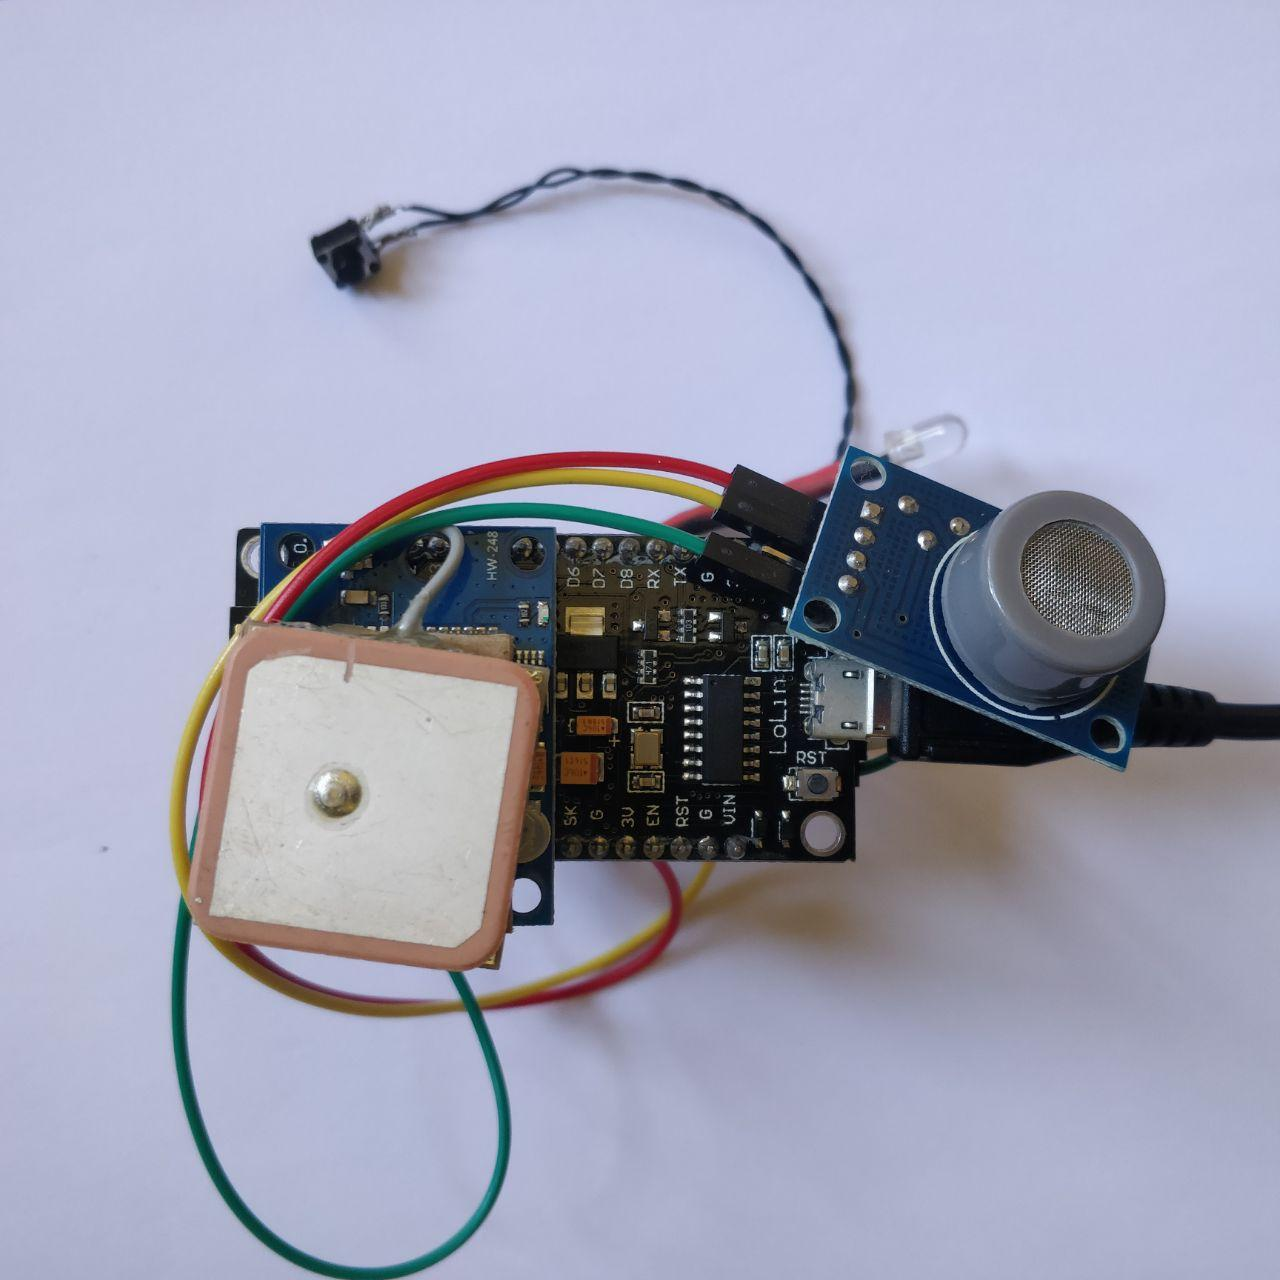
\includegraphics[width=.5\textwidth]{resources/img/ardueco_picture}
			\caption{ArduECO prototype}
		\end{figure}

	\subsection{MegaSense and Hope}
	
		% Describe the megasense project, put pictures and explain how it has been developed until now
		
%		https://www.megasense.org/
%		
%		Describe the consortium
%		
%		HOPE and Megasense
%		
%		The calibration of the megasense device is made via
%
%		MegaSense, developed at the University of Helsinki's department of Computer Science 	% Background
	%!TEX root = ../thesis.tex

\begin{savequote}[70mm]
	The Internet is becoming the town square for the global village of tomorrow.
	\qauthor{Bill Gates}
\end{savequote}


\chapter{Technologies}\label{chapter:technologies}
	
	This chapter explains more in detail the underlying technologies of this project.
	Starting from the general definition of a network and the most common architectures, to radio technologies work and then micro-controllers.
	
\section{Fundamentals of network communication}
	
	\begin{center}
		\begin{minipage}[H]{0.9\columnwidth}
			\begin{center}
				``\textit{A computer network is a structure that makes available to a data processing user at one place some data processing function or service performed at another place.}''~\cite{nla.cat-vn252493}
			\end{center}
		\end{minipage}
	\end{center}
	
	% TODO provare a citare il metaverso del zuck
	
	Starting from the definition of a computer network by Paul E. Green, it is easy to understand its importance in today's society.
	Smartphones, personal computers and other interconnected devices have become omnipresent in modern society, in which people need to feel connected to each other via these devices.
	% https://www.irishtimes.com/business/online-services-playing-more-important-role-in-everyday-activities-1.511857
	Not only they are used for fun, leisure and other social activities, but they allow connection to services such as online banking, government services and healthcare, that require a stable and secure connection among the systems that they use in order to provide a safe and sound experience for their users.
	All this to say, networks are everywhere underneath today's technology.
	There are no services or devices that can stand on their own without sharing data to other devices, to synchronize and provide a better user experience, to get updates from the manufacturer or simply to send a keep alive message.
	
	While this raw data is important for computers, people, the final users, process it to gain information, and this exchange of information from all around the world has brought radical changes many levels, from a cultural point of view to an economic point of view.
	The possibility of having a network of information exchange is the next step of globalization, which started with the exchange of goods among countries and now brings everyone together, allowing for a cultural exchange that lets people share and unite across the globe.
	
	This big network that is used to exchange information all around the world has a special name: Internet.
	% https://en.wikipedia.org/wiki/Right_to_Internet_access	
	% https://www.diplomacy.edu/blog/right-access-internet-countries-and-laws-proclaim-it/
	Many countries, such as Finland, Spain and Greece, have recognized the importance of this network and have given people the ''right to Internet access'', also known as the right to broadband or freedom to connect
	In these countries, service providers must be able to supply a mandatory minimum connection capability to all desiring home users in the regions of the country they serve.
	
	% http://www.redbooks.ibm.com/abstracts/gg243376.html
	It is important to note that Internet, with a capital I, is a particular set of worldwide interconnected networks \cite{gg243376}, but a common network of networks is called internetwork, shortened by internet, with a lowercase i.
	
	Such distinction began in the 1980s and has been described in RFCs \footnote{\href{https://datatracker.ietf.org/doc/html/rfc871}{RFC 871 (1982): A PERSPECTIVE ON THE ARPANET REFERENCE MODEL}}$^{,}$\footnote{\href{https://datatracker.ietf.org/doc/html/rfc872}{RFC 872 (1982): TCP-ON-A-LAN}} by computer scientists that understood how ARPANET was expanding and the its dimensions were not enough anymore to accommodate the amount of data traveling from one computer to another.
	% https://en.wikipedia.org/wiki/Commodore_64
	At that time, computers such as the IBM 5150 and the infamous Commodore 64 were starting to become more and more available, even if highly priced, not only to companies and universities, but also to consumers that brought them in their households, especially with the advent of MS-DOS, the dominant operating system throughout the 1980s and now open source \footnote{\url{https://github.com/microsoft/MS-DOS}}.
	
	As described by IBM in one of their technical books from the time, ''it is possible to divide the Internet such as the following groups of networks''\cite{gg243376}:
	\begin{itemize}[noitemsep]
		\item Backbones: large and strategical data routes among core networks and routers that compose and connect the Internet;
		\item Regional networks that connect large facilities such as universities and colleges;
		\item Commercial networks that provide to their subscribers access to the Internet;
		\item Local networks which run, for example, across a campus university;
	\end{itemize}

	% TODO sistemare posizione footnote alla fine
	% Oppure prendere mappa da https://www.globalbackbone.tisparkle.com/
	% Mettere riferimento a mappa interattiva
	% https://globe.gl/example/submarine-cables/
	\begin{figure}
		\centering
		\includegraphics[width=\textwidth]{resources/img/chap3/backbone}
		\caption[Subsea Internet backbone cables between US and Europe.]{Subsea Internet backbone cables between US and Europe. \footnotemark}
	\end{figure}
	\footnotetext{~\url{https://www.infrapedia.com/app}}

	Given this increase of computers connecting to the Internet, there came the need for a revised structure that could better organize these components in a more robust, but also flexible, large network.

	With more accessible OSs, such as Windows 95 and Windows 98, and the advent of Tim Berners-Lee's World Wide Web (or WWW), computers became a commodity present in many households.
	The invention of the web and its ease to navigate, using hyperlinks and search engines, culminated in the dot com bubble, a stock market bubble in the late 90s that caused rapid rise of technology companies in stock market.
	
	Networks can be categorized based on the area they cover and serve:
	\begin{itemize}[noitemsep]
		\item Wide Area Network, or WAN: sometimes called long haul networks, provide communication over long distances;
		% https://www.cloudflare.com/learning/network-layer/what-is-a-metropolitan-area-network/
		\item Metropolitan Area Network, or MAN: provide communication inside a metropolitan area, which could be a single large city, multiple cities, or any given large area with multiple buildings;
		\item Local Area Network, or LAN: provide the highest speed connections among computers in a small and circumscribed area;
		% https://www.cloudflare.com/learning/network-layer/what-is-a-personal-area-network/
		\item Personal Ara Network, or PAN: connects devices within a user's immediate area.
	\end{itemize}

	In Sec. \ref{sec:radio_tech}, is described another level of distinction based on the power consumed by the transmission medium.
	
	Since everyone can connect to the Internet and access it's services, there is no need for the average user to understand what happens between his machine and the rest of the network, which means he only sees the information that is displayed to him without knowing where it arrives from or what path it took to arrive on his monitor.
	
	% inserire immagine con la nuvoletta che si vede dentro e non si vede dentro ?
	
	For computer scientists though, it is important to understand the difference between network architecture and network topology.	
	A network architecture, as described by by Paul E. Green, ``is a complete definition of all the layers necessary to build the network''\cite{nla.cat-vn252493}.
	This is focused on the network software, which needs to be highly structure in order to allow for heterogeneous systems to communicate with each other.
	% https://standards.iso.org/ittf/PubliclyAvailableStandards/s020269_ISO_IEC_7498-1_1994(E).zip
	One example of network architecture is the ISO/OSI reference model \footnote{\url{https://www.iso.org/standard/20269.html}}, which is implemented by the TCP/IP stack of protocols.
	
	% https://stackoverflow.com/questions/38596488/in-which-layer-is-http-in-the-osi-model
	\begin{figure}[H]
		\centering
		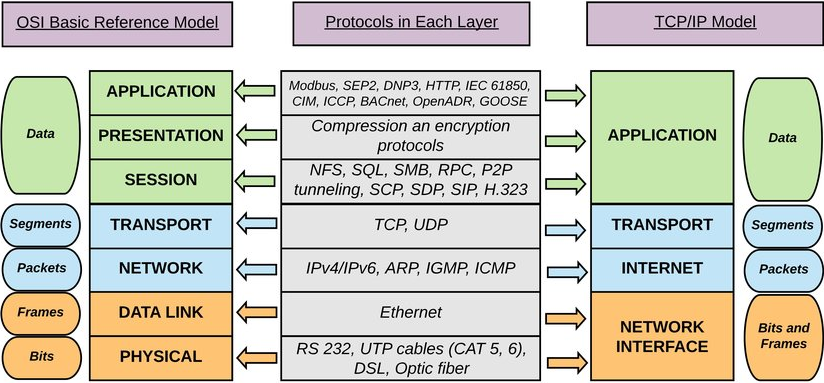
\includegraphics[width=\textwidth]{resources/img/chap3/isoosi}
		\caption{The ISO/OSI reference model against the TCP/IP stack}
	\end{figure}
	
	Thus comes the definition of a protocol as ``a set of agreements for interaction of two or more parties and is expressed by three components, syntax (e.g., a set of headers, a set of commands/responses), semantics (the actions and reactions that take place, including the exchange of messages), and timing, the sequencing and concurrency aspects of the protocol.''\cite{nla.cat-vn252493}.
	% TODO rivedere contenuto tra parentesi
	Different types of network use different architectures, based on the transmission medium and how well this performs (errors, speed, etc.).
	
	% https://www.omnisci.com/technical-glossary/network-topology
	On the other hand, the network topology refers to the manner in which the links and nodes of a network are arranged to relate to each other.
	
	\begin{figure}[H]
		\centering
		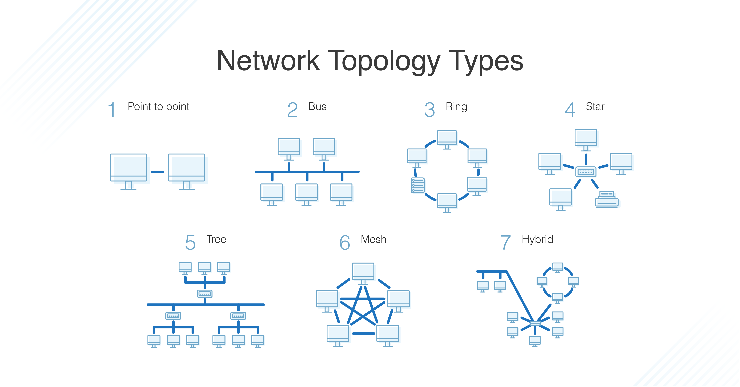
\includegraphics[width=\textwidth]{resources/img/chap3/network_topologies.png}
		\caption{Common network topologies}
		\label{img:network_topologies}
	\end{figure}
	
	As shown in Fig. \ref{img:network_topologies}, some of the most common network topologies are:
	\begin{itemize}[noitemsep]
		\item Point-to-Point: in which devices are connected directly;
		\item Bus: devices are connected to each other via a backbone cable;
		\item Ring: two dedicated point-to-point links connect a device to the two devices located on either side of it, creating a ring of devices through which data is forwarded via repeaters until it reaches the target device;
		\item Star: connects each device in the network to a central hub. Devices can only communicate with each other indirectly through the central hub;
		\item Tree: parent-child hierarchy in which star networks are interconnected via bus networks;
		\item Mesh: a dedicated point-to-point link connects each device on the network to another device on the network, only carrying data between two device;
		\item Hybrid: any combination of two or more topologies;
	\end{itemize}

	% TODO rivedere bene quando si scrive resto della tesi
	The project presented in this thesis regards a network with a mesh topology.
	This is better described in chap5 in a more depth and technical way
	The mesh proposed in this thesis has a span of LAN / MAN, since it connects devices that are in a circumscribed area but can be also placed further from each other, in order to cover longer distances.
	
	% TODO è necessaria?
	Another important distinction to make is the one between a distributed systems and a computer network.
	
	% COPIATO DA INTERNET: responsible for technical management of IETF activities and the Internet standards process
	Nowadays, the organization responsible for technical management of IETF activities and the Internet standards process is the Internet Engineering Steering Group (IESG)\footnote{\url{https://www.ietf.org/about/groups/iesg/}}.
	It is necessary to have an organization looking over the Internet itself since it gives the regulations that allow all devices to interconnect with each other.

\section{Radio technologies}\label{sec:radio_tech}
	
	% https://en.wikipedia.org/wiki/Invention_of_radio
	Although Guglielmo Marconi is usually credited as the inventor of radio due, to the creation of the first commercially successful wireless communication system \cite{4137304}, many scientists before him have studied the subject of radio waves.
	The discovery of electromagnetic waves, including radio waves, by Heinrich Rudolf Hertz in the 1880s, came after theoretical development on the connection between electricity and magnetism that started in the early 1800s.
	Scientists tried to achieve the idea of a wireless telegraph via electric conduction and electromagnetic induction for a while before the establishment of radio-based communication.
	
	% https://science.howstuffworks.com/innovation/inventions/who-invented-the-radio.htm
	Other important experiments were made by Nikola Tesla, who invented the Tesla coil, a device essential to sending and receiving radio waves, during efforts to develop a "wireless" lighting system.
	% TODO aggiungere patent?
	This Tesla coil has been used by Marconi in his experiments and is present in the patent he presented for radio transmission of data.
	
	More than a century later, radio technology has massively evolved and is used on a daily basis.
	Devices has shrunk and the amount of transmission meanings have increased far from what both Tesla and Marconi could have thought of.
	Thus, in order to give a complete picture of radio transmitting technologies, it is important to make a distinction among the ones that are made for internal or nearby use vs the ones that are used for longer distances.
	
	% https://sites.google.com/site/pnutpck11/lesson-9---wireless-transmission-media
	Many users opt for wireless transmission media because it is more convenient than installing cables, even if they might sacrifice some performance. 
	Also, using wireless technology allows transmission in locations where it is impossible to install cables.
	% TODO RIVEDERE COPIATA SPUDORATAMENTE
	Types of wireless transmission media used in communications include infrared, broadcast radio, cellular radio, microwaves, and communications satellites.
	\begin{itemize}[noitemsep]
		\item Infrared: wireless transmission medium that sends signals using infrared light waves
		\item Broadcast Radio: wireless transmission medium that distributes radio signals through the air over long distances such as between cities, regions, and countries and short distances such as within an office or home. Bluetooth, UWB, Wi-Fi, and WiMAX communications technologies use broadcast radio signals.
		\item Cellular Radio: form of broadcast radio that is used widely for mobile communications, specifically wireless modems and cell phones, which use high-frequency radio waves to transmit voice and digital data messages.
		\item Communications satellite: space station that receives microwave signals from an earth-based station, amplifies (strengthens) the signals, and broadcasts the signals back over a wide area to any number of earth-based stations.
		Applications such as air navigation, television and radio broadcasts, weather forecasting, video conferencing, paging, global positioning systems, and Internet connections use communications satellites.
	\end{itemize}
	
	With new transmission technologies, new network architectures and topologies that are better suited for the transmission method have emerged.
	Topologies that bring computation closer to the edge are also rising in popularity, since they allow for faster computation and they bring data closer to the user.
	
	LAN MAN and WAN are not enough anymore to describe the new topologies.
	An important distinction is now made by other factors such as power consumption, cost of the devices and range of the transmiter and receiver.
	
	The most important new category of wireless communication, that interests IoT and reprents a large portion of the market at the time of writing, as described in chap2, is LPWAN, which stands for Low Power Wide Area Networks.
	
	The characteristics of LPWAN are: long range, low power and low cost.
	% https://en.wikipedia.org/wiki/Low-power_wide-area_network
	Lightweight protocols reduce complexity in hardware design and lower device costs. Its long range combined with a star topology reduce expensive infrastructure requirements, and the use of license-free or licensed bands reduce network costs.

	% http://iotfactory.eu/iot-knowledge-center/overview-of-iot-networks/	
	% TODO CAMBIARE E CITARE
	% https://www.mdpi.com/1999-5903/12/3/46
	The growing popularity of IoT use cases in domains that rely on connectivity spanning large areas and the ability to handle a massive number of connections is driving the demand for LPWAN access technologies \cite{fi12030046}, and the project presented in this thesis falls under this category of communication.
	LPWAN allows connectivity in many applications, from crowded areas in smart cities to smart farming and smart environment, from security and emergencies to e-health.
	
	Various wireless transmission methods can be used to create a LPWAN, some of the most used in IoT are Sigfox, LoRa and NarrowBand IoT (NB-IoT).
	In subsection \ref{subsec:lora_lorawan}, follows a more complete explanation on LoRa and LoRaWAN.
	One important factor for all these transmission methods is to support a massive number of simultaneously connected devices with low data rates \cite{fi12030046}.
	
	Other important communication technologies in IoT are RFID, NFC, for contact purposes, Bluetooth, Zigbee for a personal network and IEEE 802.11, or WiFi, for a local area.
	The latter was used in the ArduEco project, described in chap2.
	Fig. \ref{img:wireless_coverage} contains a representation of the geographic coverage in meters of the various aforementioned wireless transmission methods.

	
	% TODO sistemare posizionamento immagine
	% \newpage
	\begin{figure}
		\centering
		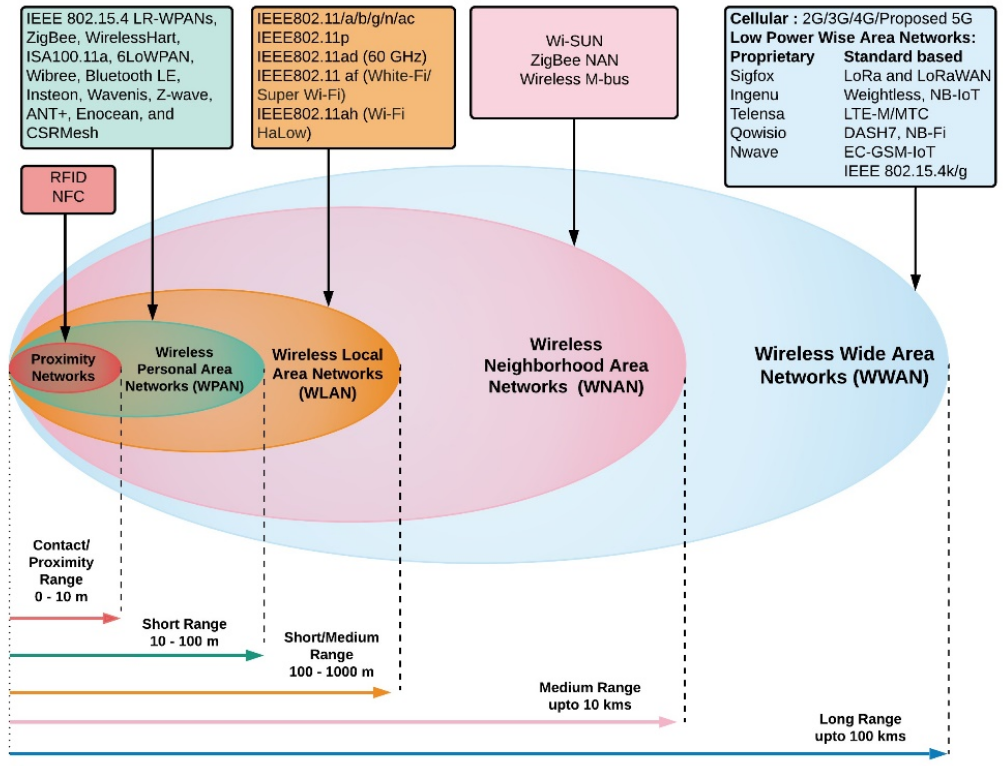
\includegraphics[width=\textheight,height=\textwidth,keepaspectratio,angle=90]{resources/img/iot_range}
		% 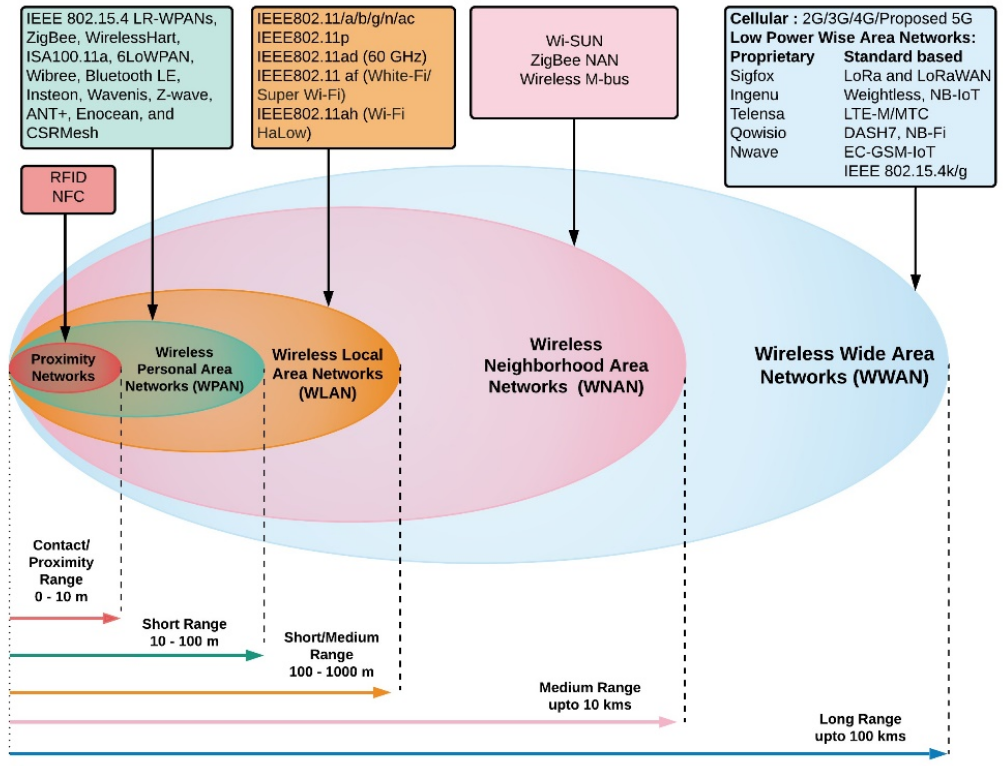
\includegraphics[height=\textwidth, angle=90]{resources/img/iot_range}
		\caption[Wireless access geographic coverage.]{Wireless access geographic coverage. \cite{fi12030046}}
		\label{img:wireless_coverage}
	\end{figure}
	% \newpage

	\subsection{LoRa and LoRaWAN}\label{subsec:lora_lorawan}
	
		% TODO modificare perchè copiato spudoratamente
		% https://www.semtech.com/lora
		LoRa (short for long range) is a spread spectrum modulation technique derived from chirp spread spectrum (CSS) technology.
		Semtech’s LoRa is a long range, low power wireless platform that has become the de facto wireless platform of Internet of Things (IoT).
		
		% https://www.design-reuse.com/news/28706/semtech-cycleo-acquisition.html
		% https://blog.semtech.com/a-brief-history-of-lora-three-inventors-share-their-personal-story-at-the-things-conference
		Since it's development in 2009, by the french company Cycleo, now acquired by the semiconductor company Semtech, LoRa has come a long way.				
		On top of it, there is a proprietary MAC protocol called “LoRaMAC”, which specifies the message formats and security layers for a true networking protocol.
		
		In February 2015, the LoRa Alliance was founded and the networking protocol was renamed “LoRaWAN.”
		% https://lora-alliance.org/
		The LoRa Alliance is a non-profit organization committed to enabling large-scale deployment of Low Power Wide Area Networks (LPWAN) IoT through the development and promotion of the LoRaWAN open standard.
		
		This organization is alike with the 3GPP 
		
		Applications of LoRa in IoT varies from smart agriculture, to smart cities, to contact tracing, to logistics and healthcare.
		A complete list of the whitepapers on LoRa based communication can be found on Semtech's official website \footnote{\url{https://www.semtech.com/lora/lora-applications}}.
		
		% TODO aggiungere tabella con specifiche
		
		\begin{figure}[H]
			\centering
			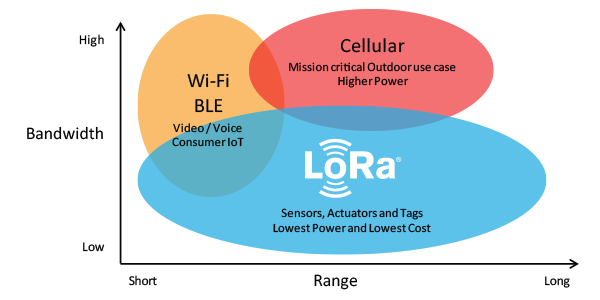
\includegraphics[width=\textwidth]{resources/img/LoRa_Why_Range}
			\caption{}
		\end{figure}

%		The smaller the package, the greater the range.
%		The greater the range, the fewer receiving antennas.
%		The fewer antennas, the lower the total costs for the user.

\section{Hardware (Microcontrollers)}\label{sec:microcontrollers}

	% Parlare di board come questa?
	% https://www.kickstarter.com/projects/sodaq/loraone-the-lora-iot-development-board?ref=discovery&term=lora%20mesh

	Microcontrollers (or MCUs, short for Microcontroller Unit) are compact integrated circuits designed to govern a specific operation in an embedded system.
	They are specially made to fit in particular environments or to perform specific functions, which usually do not require any particular computation, memory capacity or power.
	This has been made possible thanks to the continuous shrinking of transistors, which makes almost all the components more compact, and the improved power sources.
	% TODO cambiare batteries con qualcos'altro?
	In junction with the previously described wireless technologies, microcontrollers are at the hearth of IoT devices, described in Chap. \ref{chap:background}, and they require long-lasting, low-cost, and sustainable batteries.
	
	% TODO modificare un attimo
	% TODO da riprendere in chap2
	% https://ieeexplore.ieee.org/abstract/document/9148855?casa_token=ppFhpgagThgAAAAA:u81u3jhRB-EJxsnQFx32i8LI4nJBKi3NsDvemcunZKNeSETGloW8wRB45S5OeaYOOdh2kXQ
	The number of IoT connected devices is expected to grow up to 75 billion worldwide by 2025 \cite{statista}, and connection density is expected to be one million devices per square km\cite{noma}.
	These devices will generate massive data and consume significant energy.
	
	Given the amount of specific functions an MCU can perform, there are many boards on the market.
	Some are very alike, while others are very different, since they are expected to be used in other types of environments.
	All boards consist on a similar architecture, which contains the processing unit (CPU), along with memory and programmable input/output peripherals.
	
	\begin{figure}[H]
		\centering
		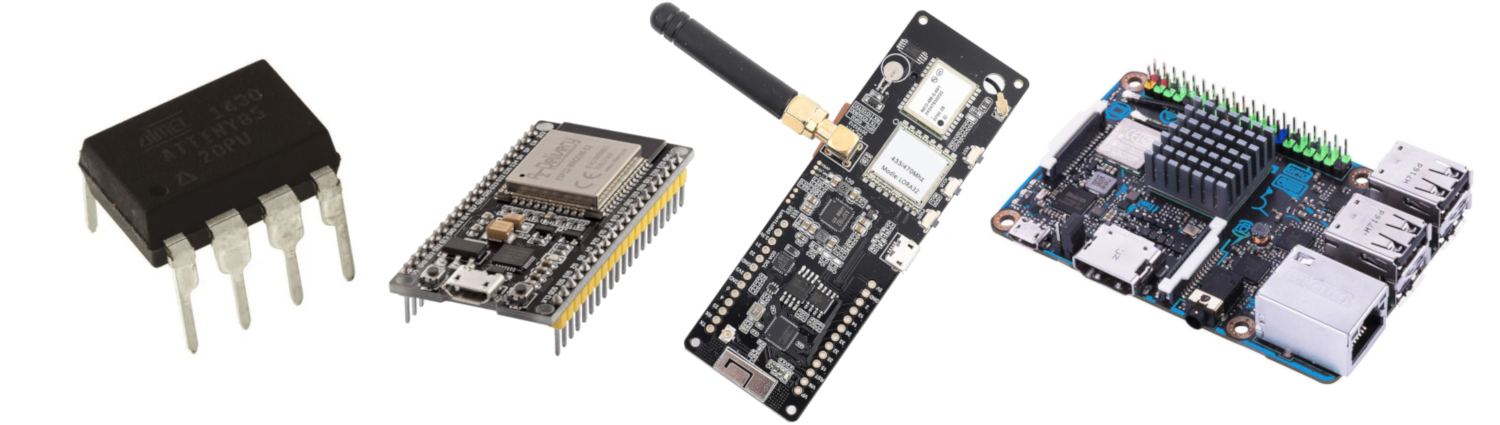
\includegraphics[width=\textwidth]{resources/img/chap3/generic_board}
		\caption{Attiny 85 on the left, in the middle two boards based on the ESP32, on the right the Asus Tinkerboard 2}
		\label{img:generic_board}
	\end{figure}

	% https://en.wikipedia.org/wiki/Microcontroller
	In Fig. \ref{img:generic_board}, there are four different boards, the one farthest on the left is the ATtiny 85 \footnote{\url{https://www.microchip.com/en-us/product/ATTINY85}}, a low-power, 8-bit microcontroller that is made for general purpose and can be programmed for simple tasks, from simple LEDs flashing, to more elaborate small sensor projects.
	% https://en.wikipedia.org/wiki/ESP32
	The two boards in the middle are based on the ESP32 chip, a series of low-cost, low-power system on a chip microcontrollers with integrated Wi-Fi and dual-mode Bluetooth.
	They both are more powerful than the ATtiny 85, and right one offers an integrated LoRa antenna on board.
	Far on the right, there is the Asus Tinkerboard 2 \footnote{\url{https://tinker-board.asus.com/product/tinker-board-2.html}}, a board powered by an Arm 6-core system on a chip (SoC), with a 64-bit Armv8 architecture.
	This board provides much more computing power compared to the previous ones and is able to run operating systems such as Linux and Windows.
	
	% https://www.amazon.it/Meipai-ATTINY85-20PU-ATTINY85-chip-ATMEL/dp/B08HPPMJ52/
	% https://www.amazon.it/AZDelivery-NodeMCU-Development-Arduino-gratuito/dp/B071P98VTG/
	% https://www.amazon.it/Scheda-Modulo-Wireless-T-Beam-Batteria/dp/B07X2KPN4L/
	% https://www.welectron.com/navi.php?qs=Tinker
	One of the strong points of these boards is the price: the ATtiny is priced around 1€ when bought in bulk, the boards on the middle cost around 7€ and 15€, while the board by Asus is the more expensive and starts from 70€.
	
	It is important to note though that using a generic board in a production environment might not be ideal, since it might lack of support and documentation.
	The boards described subsequently are from three of the major MCU producers, Arduino, Raspberry Pi and Pycom, which have built hardware that is well documented and suited for many different environments, from hobbysts to industrial use.
	
	The simplified architectures and the constraints of embedded devices are reflected in the narrow choice for programming languages.
	It is hard to find an MCU programmed in Java since this would require the JVM running in the background.
	Popular languages for MCUs are, for example, C/C++, Assembly, Rust, Ada, Erlang, etc.
	% TODO CONTROLLARE
	All these have in common the fact that they are compiled and the bytecode has a small footprint.
	A particular microcontroller company, Arduino, have developed a version of C++ specific for their boards, but given the simplictity of this new dialect, many boards on the market can be programmed with it.
	Arduino is explained further in Subsection \ref{subsec:arduino}.

	% TODO da spostare in 
	Another programming language that is quickly taking hold at the time of writing, is Mycropython.
	As explained in their website it is an "efficient implementation of the Python 3 programming language that includes a small subset of the Python standard library and is optimised to run on microcontrollers and in constrained environments" \footnote{\url{https://micropython.org/}}.
	% https://itqna.net/questions/437/what-definition-verbose-code-and-why-it-interesting-reduce-i
	Python's fast learning and explicit code advantages are reflected in this smaller version for microcontrollers, available for most of them.
	
	Below is a table with the specifications of microcontrollers from Arduino, Raspberry Pi and Pycom, which are better described in the following subsections.
	\begin{table}[htbp]
		\begin{center}
			\begin{tabularx}{\textwidth}{@{}|Y|Y|Y|Y|Y|Y|@{}} 
				\hline
				& Arduino UNO R3 & Arduino Nano BLE & Raspberry Pi & Rasperry Pi Pico & Pycom FyPy \\\hline
					CPU &&&&& \\\hline
					RAM &&&&& \\\hline
					ROM &&&&& \\\hline
					IO PINS &&&&& \\\hline
					PORTS &&&&& \\\hline
			\end{tabularx}
			\caption{Specifications of Arduino, Raspberry Pi and Pycom microcontrollers}
			\label{table:1}
		\end{center}
	\end{table}

	\subsection{Arduino}\label{subsec:arduino}
	
		% https://www.arduino.cc/en/Main/AboutUs
		% https://www.oreilly.com/library/view/arduino-a-technical/9781491934319/ch01.html	
		Arduino is a company founded by Massimo Banzi Et Al. in Ivrea, Italy, in 2005, and has released the first commercially available microcontroller.
		% TODO rivedere
		They wanted a device that was simple, easy to connect to various ''things'' (such as relays, motors, and sensors), and easy to program, besides being inexpensive.
		% It also needed to be inexpensive, as students and artists aren’t known for having lots of spare cash. 
	
		They selected the AVR family of 8-bit microcontroller devices from Atmel and designed a self-contained circuit board with easy-to-use connections, wrote bootloader firmware for the microcontroller, and packaged it all into a simple integrated development environment (IDE) that used programs called “sketches”. 
		Arduino was the result.
		
		The most famous version of their board is the UNO (one in English).
		Arduino UNO, the one on the left in Fig. \ref{img:arduino_board}, is the most used and documented board of the whole Arduino family.
		% https://www.circuito.io/blog/arduino-uno-pinout/
		Although this board does not have any integrated sensors or particular ports for peripherals.
		The current revision of the board is the Arduino UNO Rev 3 \footnote{\url{https://store.arduino.cc/products/arduino-uno-rev3}}, which consists of 14 digital pins, 6 analog inputs, a power jack, USB connection and ICSP header.
		
		% https://store.arduino.cc/products/arduino-uno-rev3
		% https://store.arduino.cc/products/arduino-yun-rev-2
		% https://store.arduino.cc/products/arduino-nano-33-ble
		\begin{figure}[H]
			\centering
			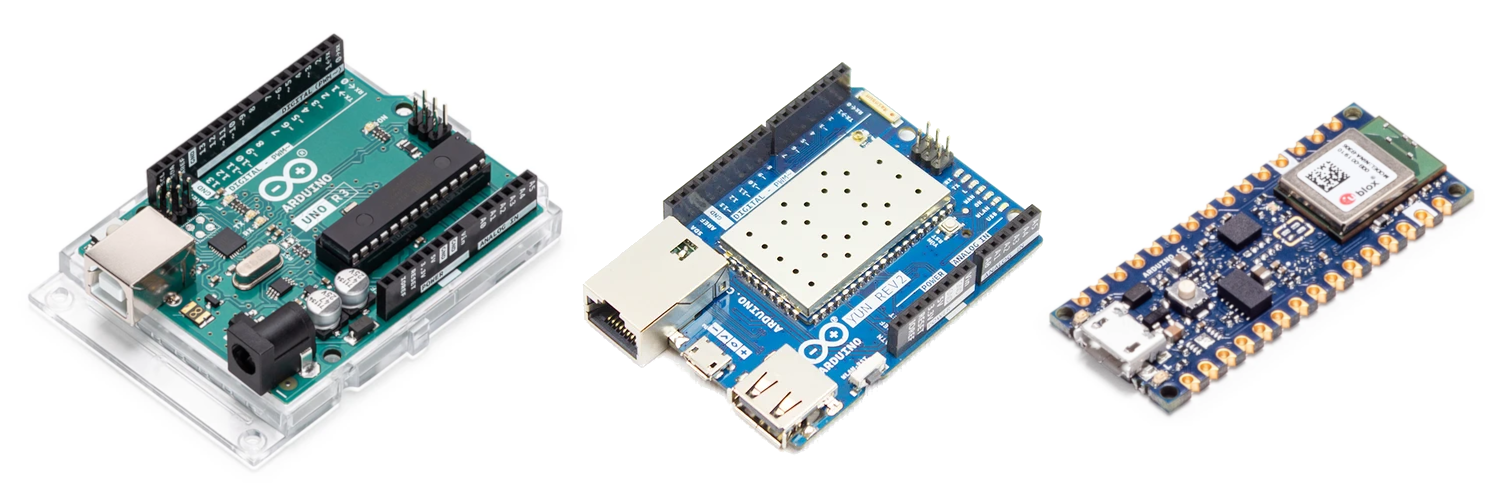
\includegraphics[width=\textwidth]{resources/img/chap3/arduino_types}
			% TODO rivedere accento yun, mettere link?
			\caption{Arduino UNO Rev 3 on the left, Arduino Yun in the middle, Arduino Nano 33 BLE on the right}
			\label{img:arduino_board}
		\end{figure}
		
		% https://www.circuito.io/blog/arduino-code/
		The Arduino family of products can be programmed in a particular programming language based on C/C++, using a special open-source integrated development environment (IDE).
		Arduino was so disruptive in the market that many boards, included the ones in Fig. \ref{img:generic_board}, support the Arduino C++.

		Shields are modular circuit boards that can be added to extend capabilities to different application needs.
		These can be attached directly on top of the board and provide sensors, interfaces, peripherals on a single board, rather than attaching to the Arduino singularly.
		% https://learn.sparkfun.com/tutorials/arduino-shields
		Some of the functionalities that can be added by a shield are Ethernet, WiFi, GPS, displays and cameras, motor drivers.
		Most of the additional shields on the market have been developed for the Arduino UNO, since it is the most common board.
		
		The choice of making the Arduino schematics open-source and accessible to anyone has largely favored the development of newer boards, similar in capacity to the Arduino but more specialized, since producers and board makers are able to keep only the components needed or add different ones.
		An example can be the two middle boards in Fig. \ref{img:generic_board}, which rode the wave of Arduino's popularity.
		Not only the datasheets are available for all boards, but also the Arduino IDE software is open-source.
		
		% https://www.circuito.io/blog/arduino-code/
		The versatility of Arduino and its simple interface makes it a leading choice for a wide range of users around the world from hobbyists, designers, and artists to product prototypes. 
		
		Newer Arduino boards offer many integrated functionalities, for example:
		\begin{itemize}[noitemsep]
			% https://store.arduino.cc/collections/boards/products/arduino-mkr-nb-1500
			\item Arduino MKR NB 1500: offers an all-in-one solution for Narrowband IoT large-coverage solutions;
			% https://store.arduino.cc/collections/boards/products/arduino-mkr-wifi-1010
			\item Arduino MKR WiFi 1010: offers integrated WiFi and Bluetooth;
			% https://store.arduino.cc/collections/boards/products/arduino-nano-33-ble-sense
			\item Arduino Nano 33 BLE Sense: contains BLE connectivity and multiple sensors, such as 9 axis inertial, humidity, and temperature, barometric, microphone, gesture, proximity, light color and light intensity.
		\end{itemize}
	
		% TODO rivedere bene quando si scrive resto della tesi
		Particularly, this last model, the board on the right in Fig. \ref{img:arduino_board}, has been considered as one of the possible choices as development board for this project.
		As better explained in chap 5, it has been discarded since it does not offer LoRa connectivity and an additional module would have been necessary to connect the board in a mesh.
							
	\subsection{Raspberry Pi}

		% https://ccclib.org/raspberrypi/
		% https://www.electronicshub.org/raspberry-pi-vs-arduino/
		Another important microcontroller on the market is the Raspberry Pi, developed by Eben Upton at the University of Cambridge in the United Kingdom with the aim of teaching and improving programming skills of students in developing countries.
		
		Compared to the Arduino specifications, it also offers more functionalities, since they include an ARM processor, a GPU with HDMI output connectivity, an Ethernet port, USB ports to connect mouse and keyboard, a camera interface, more RAM memory and more I/O pins.
		% https://www.makeuseof.com/tag/what-is-an-arm-processor/
		ARM processors, or Advanced RISC Machine processors, are better suited to mobile computing, since they use a simplified, less power-hungry method of processing.
		This allows the Raspberry Pi to run full operating systems such as some Linux distributions, included the official operating system Raspian OS
		
		% TODO rivedere perchè copiato
		Since the entire Computer (the Processor, RAM, Storage, Graphics, Connectors, etc.) is sitting on a single Printed Circuit Board, the Raspberry Pi (and other similar boards) are called as Single Board Computers or SBC.
		
		Letting their differences aside, both are very popular boards among electronics DIY builders, hobbyists and even professionals.
		Some projects involve the use of both boards in a master-slave architecture, where the Raspberry Pi acts as a master and gathers the data from the Arduinos, which are equipped with the sensors.
		
		Some of the main competitors of the Raspberry Pi are the Banana Pi and the Asus Tinkerboard (in Fig. \ref{img:generic_board}).
		Since, like the Arduino, the Raspberry Pi boards schematics are open-source and available online \footnote{\url{https://www.raspberrypi.org/documentation/computers/raspberry-pi.html}}, board makers have been able to adapt them in their own way.

		% https://en.wikipedia.org/wiki/Raspberry_Pi
		% https://www.raspberrypi.org/products/raspberry-pi-3-model-b-plus/
		
		\begin{figure}[H]
			\centering
			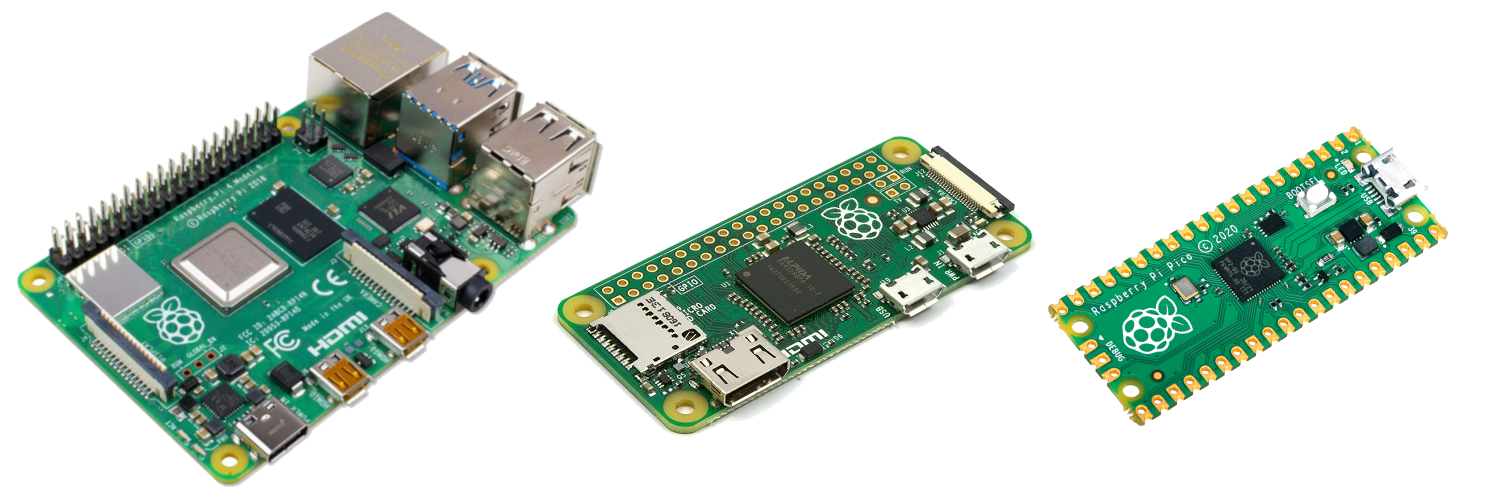
\includegraphics[width=\textwidth]{resources/img/chap3/raspberry_types}
			\caption{Raspberry Pi Model 3B+ on the left, Raspberry Pi Zero in the middle, Raspberry Pi Pico on the right}
			\label{img:raspberry_board}
		\end{figure}
		
		There are now different Raspberry Pi boards, or models, each a bit more specialized than the other.
		Some of the most important models are:
		\begin{itemize}[noitemsep]
			\item 3 B+ / 4: the model 3B+ and 4 are their most selling products, they are marketed as a ''tiny, dual-display, desktop computer'' \footnote{\url{https://www.raspberrypi.org/products/raspberry-pi-4-model-b/}};
			\item Zero: it's the smallest form factor Raspberry Pi on the market;
			\item Pico: a low-cost, high-performance microcontroller board with flexible digital interfaces.
		\end{itemize}
		
		% TODO rivedere prezzi
		They are represented in Fig. \ref{img:raspberry_board} and can be considered as the latest evolution of what is needed to learn programming in a Unix like environment at a low cost, in fact these boards cost 35\$, 5\$ and 3\$ each.
		A complete list of the available boards can be found on their online store \footnote{\url{https://www.raspberrypi.org/products/}}.
		
		% TODO rivedere bene quando si scrive resto della tesi
		The Raspberry Pi Pico was considered for this project, but was rejected since, as the Arduino, it would have needed additional modules for LoRa and BLE connectivity, while the other models have a computational power much greater than the one needed.
			
	\subsection{Pycom}
		
		% https://pycom.io/the-story-of-pycom-things/
		While Raspberry Pi and Arduino share a longer history, Pycom was founded in 2015 via a crowdfunding campaign on Kickstarter with the goal to create a new board for immediate development in the world of IoT, with all the possible connectivity.
		As the other two previously described companies, Pycom offers multiple board choices, such as the fipy, represented in Fig. \ref{img:pycom_board}, the wipy and the lopy.
		These boards are very similar to each other, since all of them offer at least WiFi and BLE, have the same chipset, interfaces and memory.
		
		\begin{figure}[H]
			\centering
			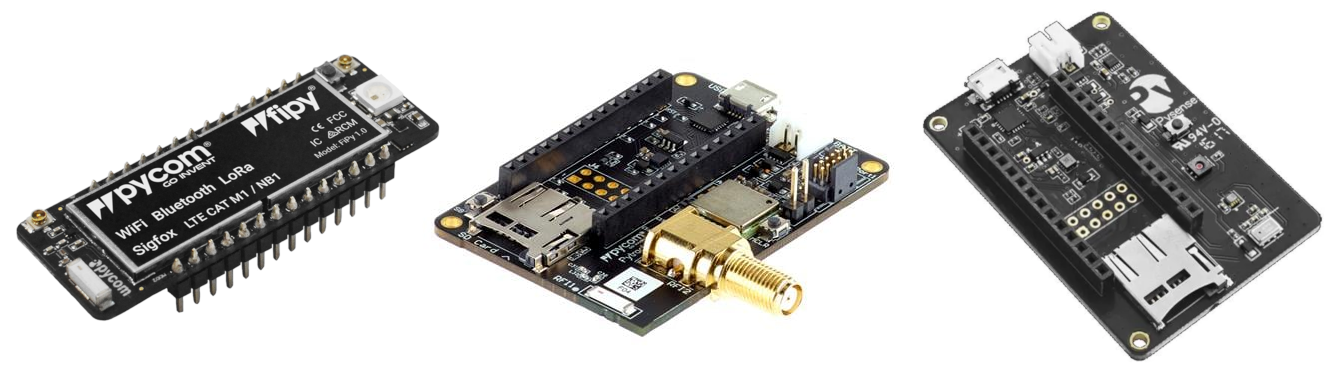
\includegraphics[width=\textwidth]{resources/img/chap3/pycom_board}
			\caption{fypy on the left, PyTrack 2X in the middle, pysense on the right}
			\label{img:pycom_board}
		\end{figure}	
		
		In particular, the FiPy board, has been chosen for this project since it packs five networks in one small board.
		As described in the product page \footnote{\url{https://pycom.io/product/fipy/}}, it is capable to communicate via WiFi, Bluetooth, LoRa, Sigfox and dual LTE-M (CAT-M1 and NB-IoT), and gives access to global LPWAN networks.
		% share similar specifications
		All the boards offered by pycom at the time of writing are equipped with an Espressif ESP32 chipset, 4MB of RAM and an flash memory of 8MB.
		
		% TODO VERIFICARE 
		% https://pycom.io/products/software/open-source/
		% https://eu.mouser.com/manufacturer/pycom/
		Contrary to Arduino and Raspberry Pi, the Pycom has decided to maintain the datasheets and the firmware of their boards proprietary, which means there is far less support from the community when comes to finding bugs in the software or improving the component placement on the board.
		Nonetheless, Pycom boards are chosen for the affability of the company producing them, also because of their high density of hardware on a board with a small footprint.
		
		Additional sensors and functions can be added to Pycom boards via shields, just like the Arduino.
		% https://pycom.io/product/pysense-2-0-x/
		% https://pycom.io/product/pytrack-2-0-x/
		Particularly for this project, the fipy has been integrated with the Pytrack 2x, which add accelerometer and GPS, and the pysense, which add ambient light, pressure and humidity.
		Both expansion boards are represented in Fig. \ref{img:pycom_board}.
				
		% https://docs.pycom.io/pybytes/
		As for the programming language, Pycom boards can be programmed using Mycropython via their Pymakr suite of IDE plugins, the Pymate mobile app, and Pybytes an online middleware platform and desktop application to remotely manage the boards.
		
		About the cost of the boards, the price of the single major components used for this project are, at the time of writing:
		\begin{itemize}[noitemsep]
			% https://pycom.io/product/fipy/
			\item FiPy €59.40
			% https://pycom.io/product/pytrack-2-0-x/
			\item Pytrack 2.0 X €40.65
			% https://pycom.io/product/pysense-2-0-x/
			\item Pysense €29.65
		\end{itemize}
		
		Although higher than an Arduino board, it is important to consider that these boards offer and all in one solution.
		The additional cost in buying an external generic shield for an Arduino board would be reflected not only on the money spent on the shield itself, but also in the time and effort of configuring and troubleshooting it in case of errors.
		An overall advantage of Pycom's products is the tight ecosystem, which allows for faster and easier troubleshooting, configuration and programming.
		All these factors are well described in Pycom's documentation on their website \footnote{\url{https://docs.pycom.io/}}.
		
		% TODO rivedere bene quando si scrive resto della tesi
		A more in depth description of how the chosen technologies interact is present in chap5.	 	% Technologies
	%!TEX root = ../thesis.tex

% https://akhiluk.medium.com/on-why-salvor-hardin-is-simply-the-best-74948711e136
\begin{savequote}[70mm]
	To succeed, planning alone is insufficient.\\One must improvise as well.
	\qauthor{Isaac Asimov, Foundation series}
\end{savequote}

%	Writing a related work section
%	https://www.seas.upenn.edu/~cse400/CSE400_2008_2009/related_work.pdf
%	Your review should: 
%	• Summarize existing research, products and systems 
%	• Talk about trends in the field 
%	• Discuss research themes that emerged from your review 
%	• Place your work in the context of cited work 
%	• Explain why the proposed project is better than or different from what already exists

\chapter{Related work}\label{chapter:related_work}

	% https://ieeexplore.ieee.org/document/7968828
	Internet  of  Things  is  one  of  the  hottest  topics  in 
	both  industry  and  academia  of  the  communication  engineering 
	world.
	% TODO citare capitolo 2 dove parlo delle aziende di iot
	On  the  other  hand,  wireless  mesh  networks,  a  network 
	topology that has been discuss for decades that haven’t been put 
	into use in large scale, can make a difference when it comes to the 
	network  in  the  IoT  world  today.

	Future IoT deployments need to focus on sustainability
	since huge centralized data centers (cloud computing) have
	become a critical part of the infrastructure.

	This chapter anticipates the one where the actual project is described and shows some related projects from which the open mesh has drawn inspiration.
	
	A  wireless  mesh  network  (WMN)  is  a  communications 
	network made up of radio nodes organized in a mesh topology 
	instead of star topology \cite{wms}.
	
	At first challenges and solutions are presented for these WMS.
	Below are also presented some of the projects which have been made at various levels from homemade projects, to research and to the ones already available on the market.
	
	\section{Challenges and solutions of wireless mesh networks}
		
		% https://beyondroot.com/blog/a-comprehensive-guide-to-mesh-network-in-iot-an-experts-take/
		
		With new technologies, wireless mesh networking has reached a point of maturity and become ideal for IoT app developers. Besides, the elevation of connected homes and industry support on open-source resources has made mesh truly accessible and low-cost. They are also regarded as much more viable and real choice for commercial as well as industrial IoT apps. At the same time, it can render extra services in a system where extending a two-node connection is limited.
		
		There are various applications for this network topology
		\begin{itemize}[noitemsep]
			\item Smart Cities: extending radio signals through campus grounds, business parks, parking garages, and other outdoor facilities
			Healthcare Equipment: monitoring and locating medical equipment. It can also serve as a backup for medical devices that always require to stay online. Thus, if one node crashes and loses connectivity, another node can step in to maintain the connection.
			\item Smart Home: You can track and manage temperature across your home using a wireless mesh network. You can also capture live data and adjust settings automatically by setting up one powered gateway, sensors, and mesh-enabled nodes in each room.
			\item Farming: Mesh networking is the best way to track sun exposure and water levels across the crops and fields. Additionally, you can create a cellular-connected IoT platform by building a mesh network across a whole acreage with the help of an IoT app development company.
		\end{itemize}

		Before choosing a mesh network topology it is important to evaluate aspects such as installation, device management and support.
		
		Energy management is an important factor as well, since the connected devices might not have a constant source of power.		
		Efficient transmission techniques and protocols that consider the amount of energy used, must be developed in order to optimally use the batteries on the devices		
		That is why there is a particular network topology, Low Power Wireless Area Network, which is focused on the interconnection of these devices
		
		Solutions to optimize the networks are being implemented both via hardware and software
		% https://ieeexplore.ieee.org/document/4068249
		Spiegare le varie soluzioni hw, dalle board migliori, e le soluzioni sw, implementazione dell'intelligenza artificiale, fare alcuni esempi e magari citare progetti presentati successivamente.
	
	\section{Overview of wireless mesh networks}
	
		% https://www.sciencedirect.com/topics/computer-science/wireless-multihop-network
		A WMS is a particular multihop network where data is sent from a node to another until it reaches its destination.
		
		\begin{figure}[H]
			\centering
			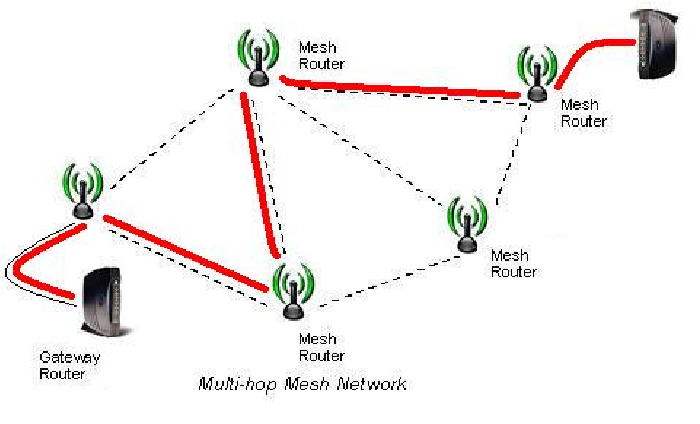
\includegraphics[width=.7\textwidth]{resources/img/chap4/mesh}
			\caption{Multihop network}
			\label{img:mesh}
		\end{figure}
		
		% https://ieeexplore.ieee.org/document/7968828
		Classic network topologies, such as the ones in Fig. \ref{img:network_topologies}, are not designed for iot networks and might not be able to meet the requirements for more dynamic devices.		
		These computer networks are not designed for low-powered devices such as remote sensors even these IoT devices are considered to be mini computers.
		The single point of failure nature of these networks makes the entire system extremely vulnerable when it comes to disasters or even difficult environment as the sensors may need to be deployed into some hardly reachable locations.Besides, the capacity of the central hub/router of the network can also limit the coverage of the service provided by IoT devices, and the range is also constrained by the same factors.
		
		An example of a multi hop wireless mesh network is VANET, a particular case of wireless multihop network, which has the constraint of fast topology changes due to the high node mobility With the increasing number of vehicles equipped with computing technologies and wireless communication devices, intervehicle communication is becoming a promising field of research, standardization, and development. VANETs enable a wide range of applications, such as prevention of collisions, safety, blind crossing, dynamic route scheduling, real-time traffic condition monitoring, etc. \cite{BADIS2015653}.
		
		Microsoft has also tried to apply mesh networking to normal internet household use \cite{bahl2009opportunistic}, however, given the improvements in telecom infrastructures and the advancement of fiber optics and internet via cable, the project has been abandoned.
		This shows how each network topology is better suited for particular scenarios.
		
		Compared to the example of microsoft's project, a vanet is more suited for a wms since the data transfered among cars is less than the one transfered among houses.
		
		\noindent
		\begin{minipage}{0.52\textwidth}% adapt widths of minipages to your needs
			\begin{figure}[H]
				\centering
				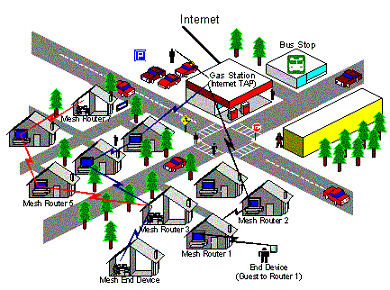
\includegraphics[width=\textwidth]{resources/img/chap4/wms_microsoft}
				\caption[Self Organizing Wireless Mesh Networks]{Self Organizing Wireless Mesh Networks \cite{bahl2009opportunistic}}
				\label{img:wms_microsoft}
			\end{figure}
		\end{minipage}%
		\hfill%
		\begin{minipage}{0.48\textwidth}\raggedright
			\begin{figure}[H]
				\centering
				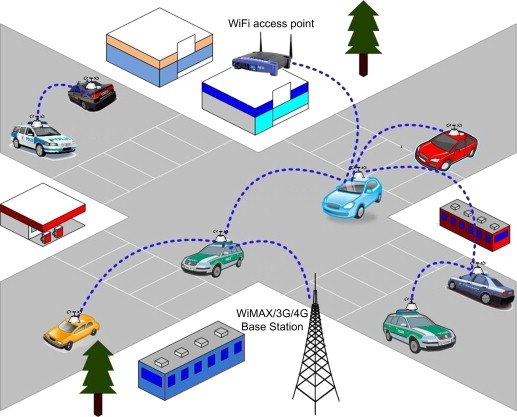
\includegraphics[width=\textwidth]{resources/img/chap4/vanet}
				\caption[An example of a VANET]{An example of a VANET \cite{BADIS2015653}}
				\label{img:vanet}
			\end{figure}
		\end{minipage}
	
		% Mesh network in other areas
		% https://www.vmware.com/products/tanzu-service-mesh.html
		
		% BLUETOOTH
		% https://www.ericsson.com/en/reports-and-papers/white-papers/bluetooth-mesh-networking
		
	
		% https://haltian.com/resource/top-four-mesh-networks/
	
		% https://www.intechopen.com/chapters/13038
	
		% https://beyondroot.com/blog/a-comprehensive-guide-to-mesh-network-in-iot-an-experts-take/
	
		\subsection{Advantages of WMS}
		
			Mesh Network for IoT devices offers enormous benefits that make it sought-after in enterprises and significant in an IoT app development company.
			Self-healing
			
			Like Shortest Path Bridging, Self-healing algorithm automatically chooses the best path to transfer data even if a few nodes lose connection. Specifically, it uses only those connections that are available and working to maintain the task.
			Self-configuring
			
			Due to auto-discovery, mesh networks are self-configuring in nature. Hence, the new nodes calibrate automatically and connect to the network without any previous setup. Consequently, network administration and expansion become easier in mesh networking.
			Scalability and Reliability
			
			In a mesh network, it is way easy to add or remove nodes without any efficiency issue. Usually, issues are in proportion to the devices. However, it is quite the opposite in the case of a mesh network. Adding nodes in a mesh network provides more routes in which data package can travel, which makes the network faster, reliable, and error-resistant.
			Cost Reduction
			
			Since mesh networks don’t require internet connection, it consumes ultra-little energy. Meanwhile, sensors are pocket-friendly and long-lasting.
			
			Besides, IoT implementation reduces expenses in many other ways like better management, optimization of resources usage, and more.
		
		\subsection{Disasvantages of WMS}
		
			Drawbacks of Mesh Network in IoT
			
			Though there are ample benefits of a mesh network, it also comes with a few drawbacks. So, it is essential to gain in-depth knowledge of this network before deciding whether a mesh network is a perfect fit for you.
			Low Capacity
			
			Mesh network is the best way of sending small data packages. Unfortunately, it doesn’t perform well while transferring video file sized data.
			
			Still, if transferring a large amount of data is compulsory, then the wifi mesh network would be a better option.
			Latency
			
			Actively switching from one node to another can decelerate the data receiving process. However, it is not an issue when your system requires a package every few minutes or so. But, it might be not enough for a few systems.
			
			Conversely, a full mesh network can accelerate the data transfer by connecting every node to one another.
			Maintenance
			
			Due to the self-healing ability of the mesh network, finding a non-working node might be time-consuming. Also, we won’t come to know if a node is having an issue.
			
			On the other hand, mesh networks for IoT devices are established to make the IoT system smarter and more efficient. So, the nodes are less prone to crash.
	
		\subsection{Scalability}
		
			% https://www.inthemesh.com/archive/the-scalability-of-mesh-networks/\\
			
			% https://ieeexplore.ieee.org/document/8071545
			
			% PAPER: LoRaWAN Range Extender for Industrial IoT
	
	\section{Algorithms for lora Wireless Mesh networks}
	
		% https://www.springerprofessional.de/en/research-on-using-the-aodv-protocol-for-a-lora-mesh-network/18715992
	
	\section{Projects}\label{sec:chap4_projects}
		
		Here are three categories of projects:
		
		\subsection{Open source projects}
		
			% https://www.hackster.io/scottpowell69/lora-mesh-chat-5267d9
			\subsubsection{LoRa Mesh Chat}\label{subsubsec:lorameshchat}

				This project consist in an add-on for mobile phones that enable text messaging in a group when outside cellular and Internet coverage.		
					
				\noindent
				\begin{minipage}{0.5\textwidth}% adapt widths of minipages to your needs
					\begin{figure}[H]
						\centering
						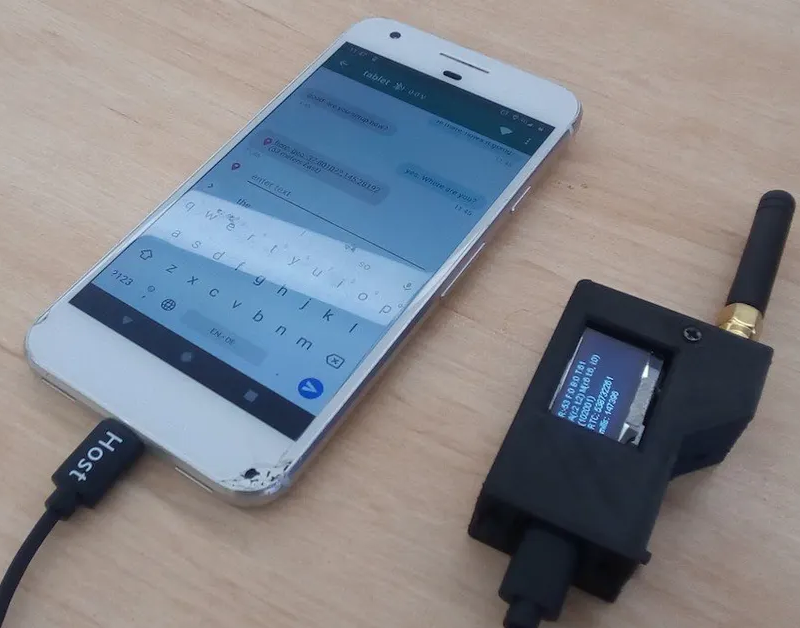
\includegraphics[width=.8\textwidth]{resources/img/chap4/lora-mesh-chat-5267d9}
						\caption{ESP32 Lora with OLED}
						\label{img:lora_mesh_chat}
					\end{figure}
				\end{minipage}%
				\hfill%
				\begin{minipage}{0.5\textwidth}\raggedright			
					As explained on the project's webpage \footnotemark, an ESP32 microcontroller with a LoRa antenna and an OLED display is programmed to connect to the phone either via and OTG cable or BLE.
					By using an application on the phone, the user is capable of sending text messages in a group.
				\end{minipage}			
				\footnotetext{{ \url{www.hackster.io/scottpowell69/lora-mesh-chat-5267d9}}}
				
				\subsubsection{Meshtastic}\label{subsubsec:meshtastic}
	
					% https://meshtastic.org/
					% https://github.com/meshtastic
					% https://www.hackster.io/punkgeek/meshtastic-a-hiking-skiing-gps-mesh-communicator-84f999
						
					Meshtastic is an open-source hiking, pilot, skiing, Signal app-extending GPS mesh communicator.
					
					Meshtastic is a project that lets you use inexpensive (\$30 ish) GPS radios as an extensible, super long battery life mesh GPS communicator. These radios are great for hiking, skiing, paragliding - essentially any hobby where you don’t have reliable internet access. Each member of your private mesh can always see the location and distance of all other members and any text messages sent to your group chat.
					
					The radios automatically create a mesh to forward packets as needed, so everyone in the group can receive messages from even the furthest member. The radios will optionally work with your phone, but no phone is required.Our device code is here, our optional Android app is here.
					
					Prebuilt binaries are included on the github sites, but it is quite easy to build from source. Instructions are included in the README. No soldering is required, essentially - buy a \$30 radio and go. We'd love to have your help extending the project - it has been super fun to work on.
		
		\subsection{Research projects}
		
			\subsubsection{Monitoring of Large-Area IoT Sensors Using LoRa Wireless Mesh Network System: Design and Evaluation}
			
			\subsubsection{Black Powder Flow Monitoring in Pipelines by Means of Multi-Hop LoRa Networks}
		
			\subsubsection{Exploring Multi-Hop LoRa for Green Smart Cities}
			
			\subsubsection{Proposal of a Hybrid LoRa Mesh / LoRaWAN Network}
			
			\subsubsection{Beyond the Star of Stars: An Introduction to Multihop and Mesh for LoRa and LoRaWAN}
			
			\subsubsection{LoRa-based Mesh Network for Off-grid Emergency Communications}
			
			% https://ieeexplore.ieee.org/document/9394317
			\subsubsection{LoRaCTP}
			
				a flexible protocol based
				on LoRa technology that allows for the transfer of “content” to
				large distances with very low energy. LoRaCTP provides all the
				necessary mechanisms to make LoRa reliable, by introducing a
				lightweight connection set-up and ideally allowing the sending
				of an as-long-as necessary data message.
			
				\begin{figure}[H]
					\centering
					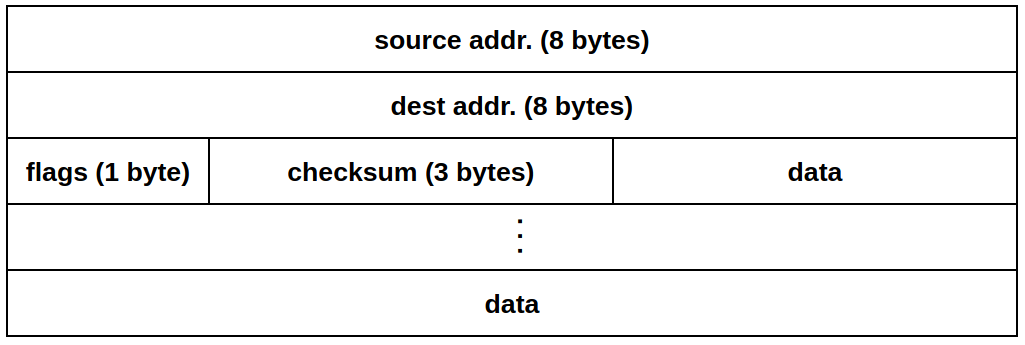
\includegraphics[width=.75\textwidth]{resources/img/chap4/loractp_packet}
					\caption[Flow of the establishment and interchange of data in LoRaCTP]{Structure of the packet used by the stop-and-wait ARQ. \cite{loractp}}
				\end{figure}
			
				\begin{figure}[H]
					\centering
					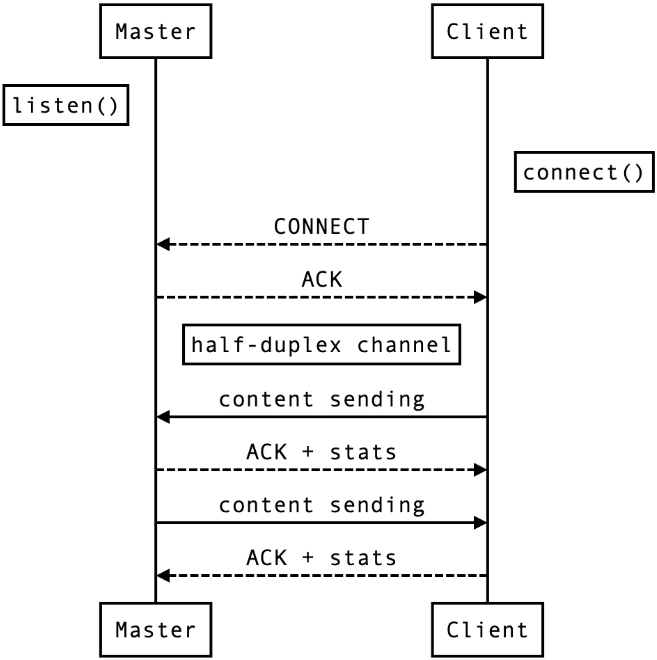
\includegraphics[width=.5\textwidth]{resources/img/chap4/loractp_flow}
					\caption[Flow of the establishment and interchange of data in LoRaCTP]{Flow of the establishment and interchange of data in LoRaCTP \cite{loractp}}
				\end{figure}
		
		By content we refer to a self-contained piece of data, like a
		JSON encoded message whose length is in principle unlimited.
		We tested out library with messages of up to 150 kbytes,
		as indicated in Section V. LoRaCTP is based on a unicast
		protocol adopting a classical stop-and-wait ARQ approach
		with a dynamic and adaptive value for the retransmission
		delay. The protocol ensures that information is not lost due to
		dropped packets and that packets are received in the correct
		order.
		
		Each packet is sent by using a three attempts scheme. That
		is, if after three attempts no ACK is received, we suppose
		that the channel is currently busy or too noisy and the content
		sending is dropped.
		
		On top of this flow-control protocol there is a lightweight
		transport protocol that is used to establish a connection be-
		tween a master node, and a client node. Figure 3 shows a sim-
		ple sequence example. Basically the master device “listens”
		to incoming connections. Connections can be established in a
		unicast manner, by providing the address of the master device,
		or using an anycast approach, thus sending to the generic
		“00000000” address and thus receiving the reply from the
		close-by listening device. This possibility allows for a greater
		flexibility in establishing dynamic topologys in rural areas, for
		example.
		
		% https://www.project-owl.com/
		% https://www.reddit.com/r/RTLSDR/comments/bzian5/ltt_showcases_new_lora_mesh_network_devices/

		\subsection{Commercial applications}

			% SONNET
			% https://www.kickstarter.com/projects/sonnet/sonnet-decentralized-mobile-communication
			% https://www.indiegogo.com/projects/sonnet-game-changer-for-wilderness-communications#/
			% GOTENNA
			% https://gotenna.com/
			%				https://gotennamesh.com/products/mesh?utm_source=internal-link&utm_medium=menu&utm_campaign=gotenna.com
			% https://techcrunch.com/2019/06/18/gotenna-is-ramping-up-public-sector-mesh-networking-with-a-24m-c-round/
			\subsubsection{Off grid mesh devices: Sonnet and goTenna}
			
				Both of the following devices use LoRa to create a mesh network and have been designed for Emergency Off-Grid Communication, where cellular towers or land-line phones are not physically reachable.
				
				\begin{minipage}{0.38\textwidth}% adapt widths of minipages to your needs
					\begin{figure}[H]
						\centering
						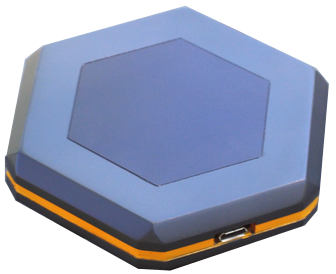
\includegraphics[width=.8\textwidth]{resources/img/chap4/sonnet}
						\caption{Sonnet}
						\label{img:sonnet}
					\end{figure}
				\end{minipage}%
				\hfill%
				\begin{minipage}{0.52\textwidth}\raggedright
					Sonnet \footnotemark, in Fig. \ref{img:sonnet}, connects to the smartphone via WiFi allowing the user to send texts, voice messages, images, data, files and share GPS locations to any other Sonnet users up to several kilometers away, thanks to LoRa.
					This completely removes smartphones' dependency on cellular grid and other network infrastructure, and allows Sonnet to be used even when there is no cellular connectivity or Internet access.
				\end{minipage}		
				\footnotetext{ \url{www.sonnettech.com}}
				\newline
			
				According to the product's Kickstarter page \footnote{ \url{www.kickstarter.com/profile/sonnet/created}} ``Sonnet's mesh network dramatically increases the effective range beyond point-to-point range by relaying data through other deices. With Sonnet, data can be relayed up to 16 times to achieve a maximum range of 80 km (50 miles)''.

				\begin{minipage}{0.5\textwidth}%
					\begin{figure}[H]
						\centering
						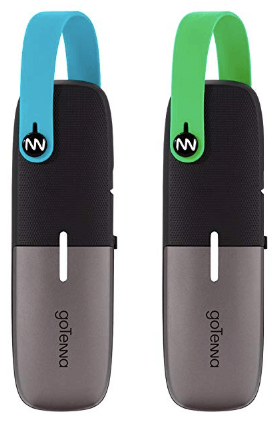
\includegraphics[height=6cm]{resources/img/chap4/gotenna}
						\caption{goTenna Mesh}
						\label{img:gotenna}
					\end{figure}
				\end{minipage}%
				\hfill%
				\begin{minipage}{0.5\textwidth}\raggedright
					\begin{figure}[H]
						\centering
						\includegraphics[width=.9\textwidth]{resources/img/chap4/gotenna_prox}
						\caption{goTenna Pro}
						\label{img:gotenna_pro}
					\end{figure}
				\end{minipage}%
				\newline
				
				The goTenna \footnote{ \url{www.gotenna.com/}}, in Fig. \ref{img:gotenna}, offers similar functions as the Sonnet, allowing to send text \& GPS locations without a cellphone with Internet connection.
				Mesh-networking allows to relay messages from a node to another until they reach destination.
				
				A compact and ruggedized network management kit, the goTenna Pro X, in Fig. \ref{img:gotenna_pro}, allows control for larger teams that operate in complex environments where no service is not an option.
						
				As Sonnet, goTenna has raised the funds necessary to enter the market as a crowdfunded project on Kickstarter \footnote{\url{www.kickstarter.com/profile/gotenna/created}}.
				
				Compared to the projects in \ref{subsubsec:lorameshchat} and \ref{subsubsec:meshtastic}, Sonnet and goTenna are more complete and offer a more stable network, thanks to the fact that these products have been thoroughly tested and produced on a bigger scale.
						
			% https://www.linksys.com/us/r/resource-center/whole-home-mesh-wifi/
			% https://www.pcmag.com/picks/the-best-wi-fi-mesh-network-systems
			\subsubsection{Mesh WiFi}
					
				Mesh WiFi, or Whole Home WiFi systems, consists of a main router that connects directly to the main modem, and a series of satellite modules, or nodes, placed around the house for full WiFi coverage.
				Each node serves as a hop point for other nodes in the system and are all part of a single wireless network and share the same SSID and password, unlike traditional WiFi routers.
				Weakened signal or WiFi dead spots of the latter are the result of physical obstructions (floor, doors, and walls).
				
				A modular mesh whole home WiFi system is flexible and scalable, giving a customizable method of expanding WiFi coverage without the need to add range extenders, which are certainly effective when it comes to increasing the router range, but they do so at the expense of WiFi performance, which gets cut in half.
				
				It’s just like installing lighting fixtures to illuminate your home; you can place your nodes anywhere in your home. You choose which rooms need the coverage, and when it’s time to add more to extend the signal even further. 				
			
				\begin{figure}
					\centering
					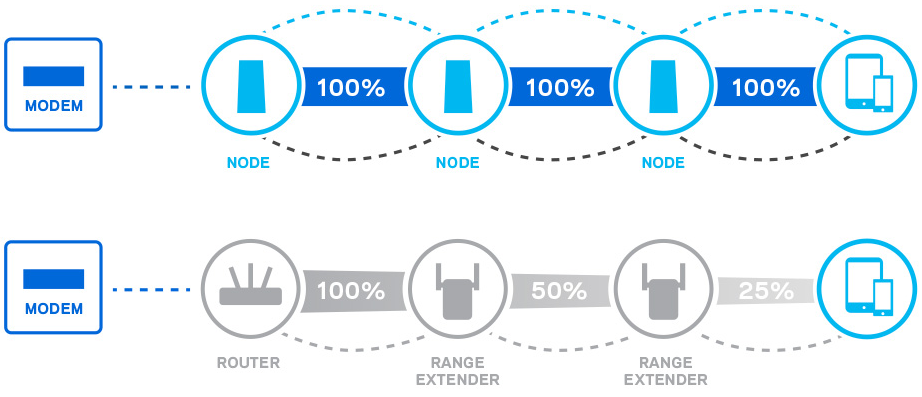
\includegraphics[width=\textwidth]{resources/img/chap4/wifi6}
					\caption{WiFi 6 mesh nodes vs WiFi range extenders performance}
					\label{img:wifi6}
				\end{figure}
				
				Wi-Fi 6 is an evolution of 802.11ac technology that promises increased throughput speeds (up to 9.6Gbps), less network congestion, greater client capacity, and better range performance thanks to the new and improved wireless technologies, including Orthogonal Frequency-Division Multiple Access (OFDMA). OFDMA improves overall throughput by breaking Wi-Fi channels into sub-channels, allowing up to 30 users to share a channel at the same time. Additionally, 802.11ax takes advantage of previously unused radio frequencies to provide faster 2.4GHz performance and uses MU-MIMO streaming, too. Some Wi-Fi 6 devices can also communicate on the less-crowded 6GHz band, which was recently opened for Wi-Fi and is known as Wi-Fi 6E.
				
				Many important manufacturers for network hardware, like Netgear and Cisco, have already implemented such technology and functions in their products.
						
						
%			% https://docs.pycom.io/pymesh/
%			% https://pycom.io/pymesh-relaunch/
%			\subsubsection{pymesh}
%			
%				Pycom itself has an available mesh network that connects lora devices, compared to the one proposed in this paper thought
%
%				
%				
%				Pymesh is the LoRa full-mesh network technology.
%				
%				A Mesh network acts like a net, this means that any node within the network can connect with any other node.
%				
%				Mesh networks essentially get rid of gateways, which decentralises the network’s infrastructure. This then means that the network becomes flexible, so it can do many wonderful things – such as generate, change and fix itself. The success of the Mesh network is down to its parts, as any node within the network will automatically connect to the best radio-link available.
%				
%				Pymesh works on all of our LoRa supporting development boards, the LoPy4 and FiPy as well as on our OEM modules, L01 and L04.
%				
%				An ad-hoc communication network over raw-LoRa radio
%				Multi-gateway (Border Routers) Nodes that connect Mesh-internal data with the Cloud
%				Each Node uses LBS - Listen Before Talk
%				Security on multiple levels
%				base level: authentication and encryption using AES 128bit key, so all traffic inside Pymesh is secured
%				advanced level: RSA or AES at application level allows private communication channels above Pymesh.
%				Any LoRa device (Lopy4/Fipy) can have any of the Pymesh Node Role: Leader, Router, Child or Border Router
%				
%				What does Pymesh integration offer you?
%				
%				This documentation is a quick introduction to the new Pymesh integration features on Pybytes.
%				
%				The Pymesh integration is here to help Pymesh firmware deployment and to monitor Pymesh node’s health
%	
%	
%				
%				
%				Mesh networks essentially get rid of gateways, which decentralises the network’s infrastructure. This then means that the network becomes flexible, so it can do many wonderful things – such as generate, change and fix itself. The success of the Mesh network is down to its parts, as any node within the network will automatically connect to the best radio-link available.
%				
%				
%				PROS and CONS of this mesh 	% Related work
	%!TEX root = ../thesis.tex

% https://en.wikipedia.org/wiki/Kelly_Johnson_(engineer)
% https://en.wikipedia.org/wiki/KISS_principle
\begin{savequote}[40mm]
	\textbf{K}eep\\
	\textbf{I}t\\
	\textbf{S}imple\\
	\textbf{S}tupid
	\qauthor{Kelly Johnson}
\end{savequote}

\chapter{Proposed solution}\label{chapter:proposed_solution}

	This chapter contains the technical description of ``\textit{Open LoRa Mesh}'', a mesh network composed by FiPy devices that communicate with each other via LoRa.
	Open LoRa Mesh is able to accommodate small messages, such as the ones sent by MegaSense, described in Section~\ref{subsec:megasense}.
	All network related functions are contained in a library that describes main components of this project.

	Even though it would have been possible to use a simulator, such as ``\textit{The one}''\footnote{ \url{akeranen.github.io/the-one}}, for demonstrating the usefulness of such network, the final project has been realized with Pycom hardware, discussed in Section~\ref{sec:hardware_solution}.
	
	The code created for this project is open sourced and available on GitHub under the repository \textit{Open LoRa Mesh} \footnote{ \url{www.github.com/cipz/OpenLoRaMesh}}, and better explained in the following Section~\ref{sec:software_solution}.
	
	\section{Network architecture}\label{sec:architecture}
		
		Before talking about the architecture of Open LoRa Mesh, it is important to understand the one of the MegaSense.
		As can be seen in Figure~\ref{img:megasense_architecture}, since each MegaSense device is made to be carried by a person, devices connect each one to the user's phone.
		The latter then communicates with the MegaSense and, via the application developed by the Computer Science Department at the University of Helsinki, sends the air-quality readings and the GPS location, which has been read by the application from the phone itself, to the servers in the cloud.
		
		Communication between MegaSense and phone is done via BLE, and exchanges data such as sensor readings (like NO2,
		O3, CO, battery percentage, \textit{etc.}) and calibration measurements, in \texttt{JSON} format.
		Thus each device has to be linked to a person's phone, which might enhance the portability of the device, but not its possibility to read data independently if placed in a specific location.
		Such communication resembles the one from devices described in Section~\ref{subsec:commercial_applications}.
		
		\begin{figure}[h]
			\centering
			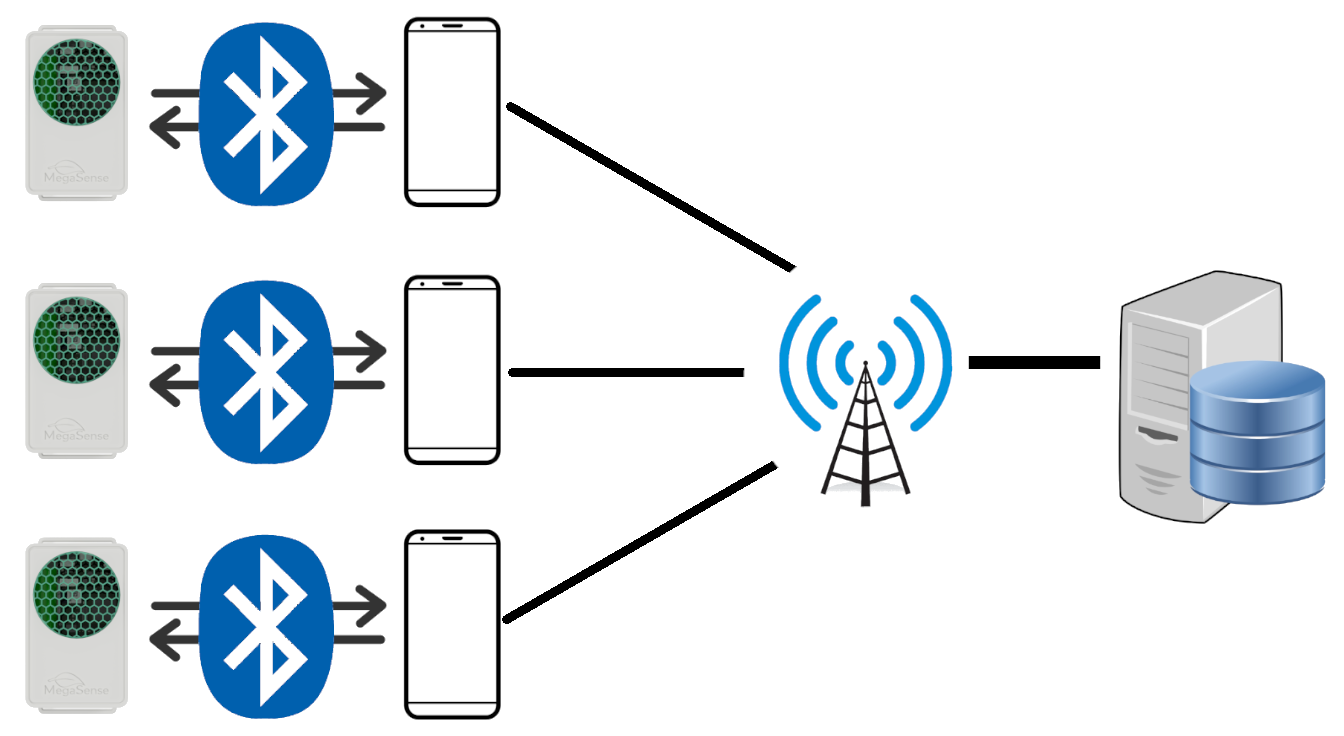
\includegraphics[width=.75\textwidth]{resources/img/chap5/architecture_megasense}
			\caption{MegaSense architecture}
			\label{img:megasense_architecture}
		\end{figure}
	
		One of the goals Open LoRa Mesh tries to achieve is to give independence to these devices so that they can communicate with one another and allow information to be passed along between nodes without the aid of a user's phone.
	
		This is why the architecture would evolve from the one in Figure~\ref{img:megasense_architecture} to Figure~\ref{img:openmesh_architecture}: the phone is replaced by a FiPy, which also connects to the MegaSense via BLE, and sends the data acquired from the sensors in the network.
		Nodes communicate with each other via LoRa, detailed in Section~\ref{subsec:lora_lorawan}, and exchange data using mainly \textit{LoRaCTP}, described in Section~\ref{subsec:loractp}.
		
		\begin{figure}[h]
			\centering
			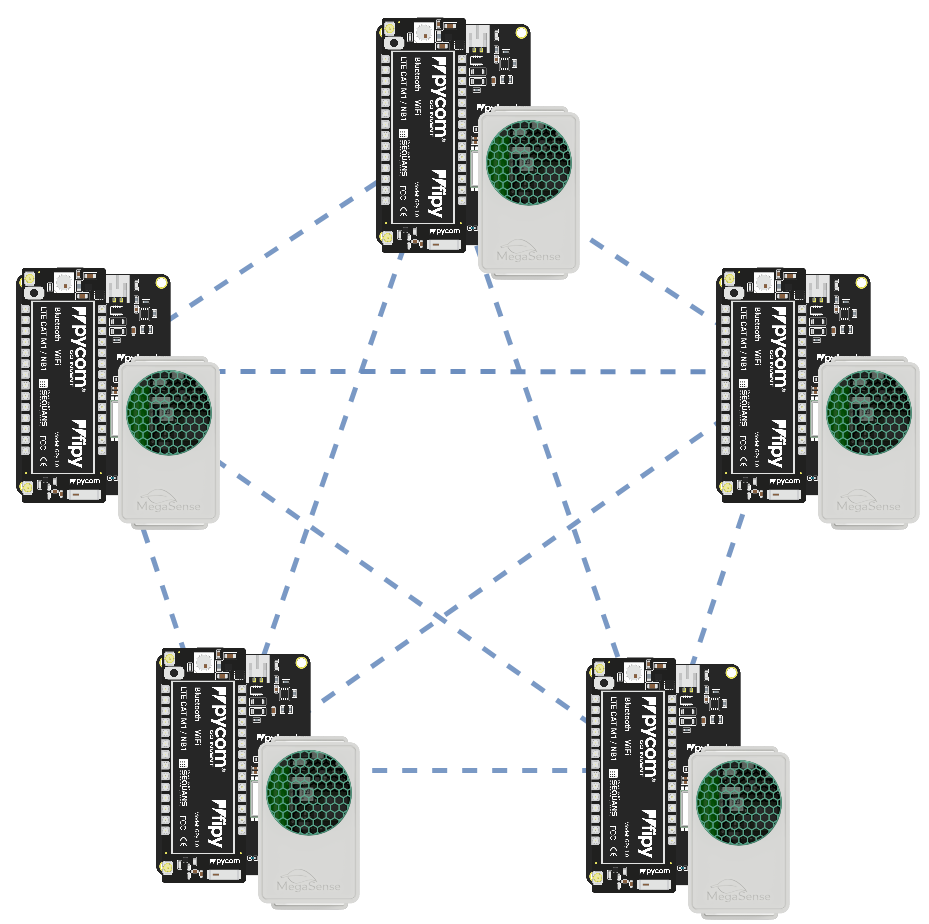
\includegraphics[width=.7\textwidth]{resources/img/chap5/mesh-architecture-1}
			\caption{Open LoRa Mesh architecture}
			\label{img:openmesh_architecture}
		\end{figure}
		
		Each FiPy board represents a node of the network, which in this case is a ``\textit{Flat Wireless Mesh}'', where each node acts both as data provider and as data forwarder.
		Although simple, such network architecture is well known from the previously mentioned, Section~\ref{sec:scalability}, Gupta and Kumar \cite{825799}.
		Besides not scaling well and having the potential to put very high resource constraints, ``\textit{addressing schemes and service discovery would prove to be a major bottleneck against scalability}'' \cite{92000412}.
		
		Despite having these disadvantages, it is important to keep in mind the small environment and the limited number of devices that will be connected in such network.
		Since communication is not frequent and data packets are not large, this network layout can satisfy the MegaSense's requirements for interconnection.

	\section{Open LoRa Mesh Hardware}\label{sec:hardware_solution}
	
		For the development of Open LoRa Mesh, the chosen hardware to replace the phone in the original MegaSense architecture is composed by Pycom's FiPy microcontrollers, along with its shields, like the PyTrack and the PySense.
		A prototype of the MegaSense device was also given from the developers of the project in order to test the connectivity with the Pycom boards and test its capacity to send and receive data from other nodes in the network.
		All devices can be seen together in Figure~\ref{img:irl_picture_1}.
		
		\begin{figure}[h]
			\centering
			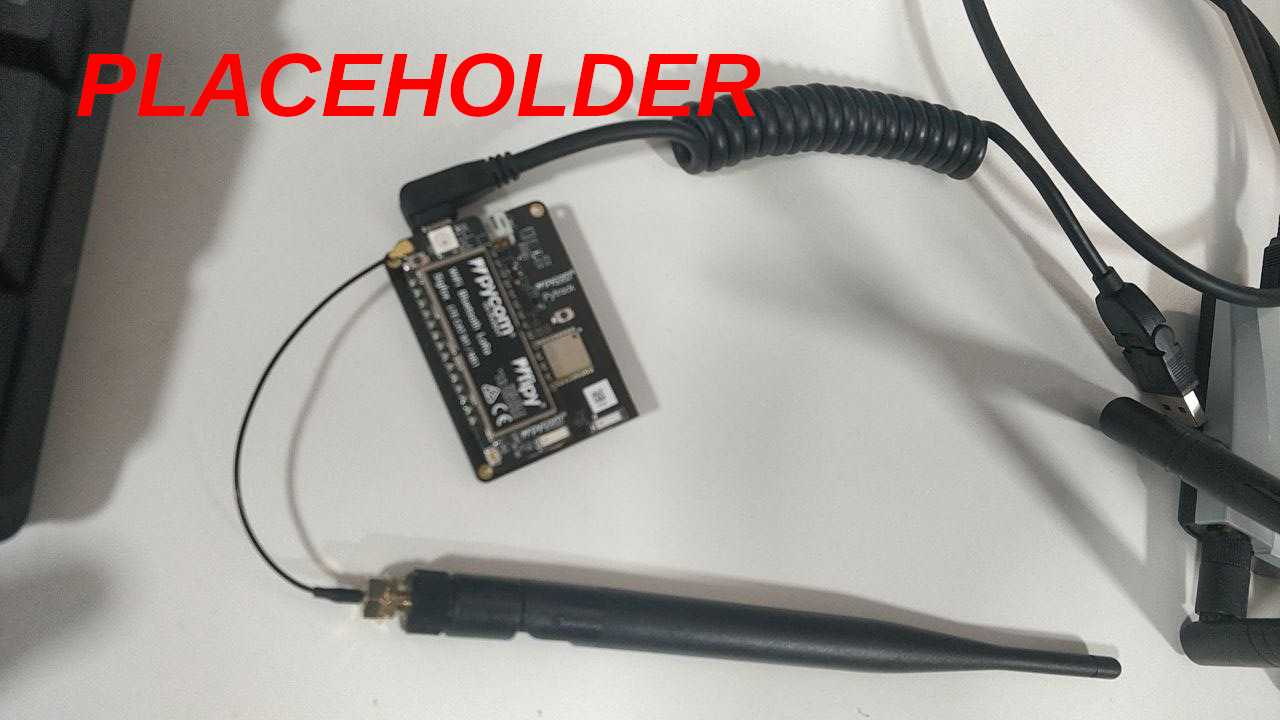
\includegraphics[width=\textwidth]{resources/img/chap5/mesh-irl-picture}
			\caption{FiPy with PyTrack, LoRa antenna, GPS antenna and MegaSense prototype}
			\label{img:irl_picture_1}
		\end{figure}
		
		Although the expansion board is important, the FiPy is the one that contains all the chips that allow connectivity, as said in Section~\ref{sec:pycom}.
		After an initial evaluation on the requirements necessary in creating a network for exchanging messages among air quality sensing devices, Pycom's boards have come first considering the numerous possibilities it allows for prototyping.
		
		The exact hardware with which this project has been completed is: four FiPy boards, one PyTrack 2X, one PyTrack, two PySense shields and one MegaSense prototype, Figure~\ref{img:megasense_picture}.
		Pycom boards do not have a USB connection directly on them, so they can be programmed either using a shield or via an UART (Universal Asynchronous Receiver-Transmitter) to USB.
		
		Alternative microcontrollers, such as the Raspberry Pi Pico, Raspberry Pi 4, Arduino Nano 33 BLE Sense, and ESP32 boards have been discard given either their excessive power or their need for multiple expansion shields.
				
	\section{Open LoRa Mesh Software}\label{sec:software_solution}
	
		While Arduino's C++ dialect divides the code in two main functions, the \texttt{setup()} and \texttt{loop()}, as mentioned in Chapter~\ref{chapter:technologies}, the Pycom boards use two files to separate an initial bootstrap of the board and a main section of the code.
		These two special files are called \texttt{boot.py} and \texttt{main.py} respectively.
		
		The following section explains the algorithms made for this project are delineated and it is shown how they have been implemented.
		Afterwards, the addressing scheme in LoRa, which is important to understand, is described.
		
		All network related functions are contained in a library that describes main components of this project.
		
		The FiPy boards have been programmed using Micropython, and the firmware flashed\footnote{ \textit{Flashing} involves the overwriting of existing firmware or data, contained in EEPROM or flash memory module present in an electronic device, with new data.} on the boards, at the time of writing, is \texttt{v1.16.5}.
		
		\subsection{Important functions}\label{subsec:algorithms}
	
			% DRAWING AUTOMATA
			% https://latexdraw.com/automata-diagrams-in-latex/
			% https://hayesall.com/blog/latex-automata/
			
			% DRAWING FLOWCHART
			% https://www.overleaf.com/learn/latex/LaTeX_Graphics_using_TikZ%3A_A_Tutorial_for_Beginners_(Part_3)%E2%80%94Creating_Flowcharts

			This subsection shows in depth how the software works, for more significant building block of the code there are finite-state automata (or FSA) that show the state nodes find themselves in.
			For a graphical reason, each state of the following automata is abbreviated, and, when needed, the full state is described in a table underneath it.
			
			At first an overview of the entire software is presented, then for each important component of the software there is a subsection that describes how it functions and connects to the rest.
			Such vision should allow to understand the system from a broader point of view to a more detailed one, where every function is analyzed.
			
			\subsubsection{Overview of the whole system}
			
				As previously said, the FiPy is divided in two files, \texttt{boot.py} and \texttt{main.py}.
				When the board is powered up, the first file executed is \texttt{boot.py}, which contains the code that either boots the device in a state of receiver or continues its normal sequence.
				
				The receiver state allows for the device to be used as a station that only sniffs the messages traveling in the air.				
				Continuing in the normal sequence, thus executing the code in \texttt{main.py}, will allow the node to connect to an existing mesh or to create one, for sending and receiving data afterwards.
				
				Open LoRa Mesh heavily relies on the use of LoRaCTP, described in Section~\ref{subsec:loractp}, for message transmission.
				This is because LoRaCTP builds an important layer of stability on top of raw LoRa transmission.
				
			\subsubsection{Boot sequence}
			
				As mentioned earlier, the \texttt{boot.py} file contains the code that is initially executed by the FiPy.
				The first operation done is to disable Wi-Fi communication and the default blinking (heartbeat) of the FiPy, Figure~\ref{code:boot_wifi}.
				Since when powered up, FiPy's firmware enables Wi-Fi, it can be useful to turn it off because it is not used, also it could draw unnecessary power from the device.

				\begin{figure}[H]
					\begin{lstlisting}[language=Python]
wlan = WLAN(mode=WLAN.STA)
wlan.deinit()
pycom.heartbeat(False)
					\end{lstlisting}
					\caption{Code for Wi-Fi de-initialization and heartbeat stop}
					\label{code:boot_wifi}
				\end{figure}
			
				During the boot procedure, the board checks the availability of a \texttt{config.json} file on an external SD card and, if present, uses the parameters on such files.
				If not present it checks for such file locally on the flash memory, which contains one with default configurations and is uploaded with the \texttt{*.py} files.

				The configuration file contains the custom parameters that can be used by the board, and
				include \texttt{BOOT\_MODE}, which can either be \texttt{DEFAULT\_BOOT} or \texttt{PLAIN\_RECEIVER}.
				If set to \texttt{DEFAULT\_BOOT}, the board will normally proceed to executing the software in \texttt{main.py}.
				When set to \texttt{PLAIN\_RECEIVER}, the board will execute code which makes it listen to the packets traveling in the air.
				Such process can be seen in Figure~\ref{fsa:boot_sequence}, described in Table~\ref{table:fsa_boot}
				
				Other modes could be added to the software as an improvement, but at the time of writing only these have been implemented.
				Improvements on this topic is later about in Section~\ref{sec:software_improvements}.
									
				\begin{figure}[h]
					\centering
					\begin{tikzpicture}[shorten >=1pt,node distance=2cm,on grid,auto]
					
					% Help grid
					% \draw [help lines] (-1,1) grid (6,-6);
					
					\tikzstyle{every state}=[fill={rgb:black,1;white,5}]
					
					
					\node[state, initial]  			(s_0)                 	{$s_0$}; % START
					\node[state] 					(s_1)	[right of=s_0]	{$s_1$}; % BOOT
					\node[state, accepting]			(s_2) 	[above right of=s_1]	{$s_2$}; % MAIN LOOP
					\node[state, accepting]			(s_3) 	[below right of=s_1]	{$s_3$}; % RECEIVER LOOP
					
					\path[->]
					(s_0) edge node {} (s_1)
					(s_1) edge node {} (s_2)
					(s_1) edge node {} (s_3)
					(s_2) edge [loop right] node {} ()
					(s_3) edge [loop right] node {} ();
					
					\end{tikzpicture}
					\caption{FSA for the overview of boot sequence}
					\label{fsa:boot_sequence}
				\end{figure}				
		
				\begin{table}[h]
					\begin{center}
						\begin{tabular}{|c|m{10.2cm}|} 
							\hline
							\textbf{State abbreviation} & \textbf{State description} \\\hline
							$start$ & device is powered up\\\hline
							$s_{0}$ & Wi-Fi is de-initialized and heartbeat is set to \texttt{False}\\\hline
							$s_{1}$ & configuration file is read\\\hline
							$s_{2}$ & \texttt{PLAIN\_RECEIVER} mode is initialized\\\hline
							$s_{3}$ & \texttt{DEFAULT\_BOOT} mode is initialized\\\hline
						\end{tabular}
						\caption{Boot sequence FSA description}
						\label{table:fsa_boot}
					\end{center}
				\end{table}

			\subsubsection{Plain receiver}
			
				The mode in which the device is set only to listen is called ``\textit{\texttt{PLAIN\_RECEIVER}}'', and the code executed is contained in the \texttt{plain\_receiver.py} file.
				Such state lets the FiPy listen to messages that are in its range, without the possibility of sending messages or participate into the mesh.
				This state can be used for debugging and catching the different messages that are sent in an area.
				
				\begin{figure}[H]
					\begin{lstlisting}[language=python]
def sniffLoRaNetwork():
  ctpc = loractp.CTPendpoint()
  print("Executing plain_receiver.py")
  while True:
    print('plainreceiver.py: waiting for data')
    try:
      rcvd_data, addr = ctpc.recvit()
      print("plainreceiver.py: got {} from {}".format(rcvd_data, addr))
    except Exception as e:
      print ("plainreceiver.py: EXCEPTION!! ", e)
					\end{lstlisting}
					\caption{\texttt{PLAIN\_RECEIVER} mode code}
					\label{code:plain_receiver}
				\end{figure}

				The principal function in the file \texttt{plain\_receiver.py} is \texttt{plain\_receiver()}, in Figure~\ref{code:plain_receiver}.
				Such function is an adaptation of the example one contained in the LoRaCTP repository.
				It first creates an endpoint, which is then used in an infinite loop that reads data received at the endpoint and logs it.
				
			\subsubsection{Main sequence and key variables}
			
				This subsection describes the course of the \texttt{main.py} file and the \texttt{main()} function it contains.
				The code contained in this file is automatically executed by the board, unless specified otherwise, after the code in the previously described \texttt{boot.py} file.
				
				\begin{figure}[h]
					\centering
					\begin{tikzpicture}[shorten >=1pt,node distance=2cm,on grid,auto]
					
					% Help grid
					% \draw [help lines] (-1,1) grid (6,-6);
					
					\tikzstyle{every state}=[fill={rgb:black,1;white,5}]
					
					
					\node[state]  					(s_3)                 	{$s_3$}; % PICKS UP FROM BOOT
					\node[state] 					(m_0)	[right of=s_3]	{$m_0$}; % INITIALIZE VARIABLES AND OBJECTS AND LOCKS THE LORA ANTENNA AND CREATES CONNECTION WITH MEGASENSE, IF AVAILABLE
					\node[state]					(m_1) 	[right of=m_0]	{$m_1$}; % LISTEN LOOP FOR MESSAGES OF EXISTING LORA MESHES
					\node[state]					(m_2) 	[above right of=m_1]	{$m_2$}; % LORA MESH EXISTS
					\node[state]					(m_3) 	[below right of=m_1]	{$m_3$}; % LORA MESH DOES NOT EXIST, CREATE NEW MESH
					\node[state,accepting]			(m_4) 	[above right of=m_3]	{$m_4$}; % NODE LISTENS FOR MESSAGES IN THE AIR AND ANALYZES IT
					\node[state]					(m_5) 	[right of=m_4]	{$m_5$}; % IF AVAILABLE COMMUNICATES WITH MEGASENSE AND READS DATA FROM IT
					\node[state]					(m_6) 	[right of=m_5]	{$m_6$}; % COMMUNICATE WITH MEGASENSE
					
					\path[->]
					(s_3) edge node {} (m_0)
					(m_0) edge node {} (m_1)
					(m_1) edge [loop above] node {} ()
					(m_1) edge node {} (m_2)
					(m_1) edge node {} (m_3)
					(m_3) edge node {} (m_4)
					(m_2) edge node {} (m_4)
					(m_4) edge node {} (m_5)
					(m_5) edge node {} (m_6)
					(m_6) edge [bend left] node {} (m_4);
					
					\end{tikzpicture}
					\caption{FSA for the overview of the main code}
					\label{fsa:main}
				\end{figure}		
			
				\begin{table}[h]
					\begin{center}
						\begin{tabular}{|c|m{10.2cm}|} 
							\hline
							\textbf{State abbreviation} & \textbf{State description} \\\hline
							$s_{3}$ & state $s_{3}$ from Figure~\ref{fsa:boot_sequence} where the code \texttt{main.py} starts\\\hline
							$m_{0}$ & variables,objects and communication with MegaSense device, if available, are initialized\\\hline
							$m_{1}$ & listen loop for messages for existing LoRa mesh network\\\hline
							$m_{2}$ & if the mesh exists, the node exchanges information about it with the advertising node\\\hline
							$m_{3}$ & if the mesh does not exist, the node creates a new mesh and advertises the mesh information\\\hline
							$m_{4}$ & the node listens for any messages in the air and processes them\\\hline
							$m_{5}$ & if the MegaSense device is available, the node connects to it, reads data, and sends it into the network\\\hline
							$m_{6}$ & the node broadcasts a message advertising the mesh network\\\hline
						\end{tabular}
						\caption{Main sequence FSA description}
						\label{table:fsa_main}
					\end{center}
				\end{table}
			
				The most important objects used in the main part of this software, and that are initialized at the beginning, are:
				\begin{itemize}
					\item \texttt{LORA\_ANTENNA\_LOCK}: a \texttt{LOCK} is placed on the use of the LoRa antenna so that it can be used only in one part of the program at the time; 
				    \item \texttt{node}: represents the current node and its properties;
					\item \texttt{mesh}: contains the data about the mesh network;
					\item \texttt{routing\_table}: contains data about the other nodes connected to the mesh.
				\end{itemize}
			
				\texttt{node}, \texttt{mesh} and \texttt{routing\_table} are all objects initialized from the \texttt{mesh.py} library, later described in Section~\ref{subsec:mesh_library}.
				
				Like in the \texttt{boot()} function, \texttt{main()} also searches for a configuration file, at first on an SD card, then on the flash memory.
				Important entries in this \texttt{JSON} file used by \texttt{main()} are:
				\begin{itemize}
					\item \texttt{GPS}: a boolean that tells the FiPy to either find or not the GPS coordinates of the board. This only happens if the board is connected to a PyTrack shield;
					\item \texttt{MEGASENSE\_CONNECT}: another boolean that tells the board either to connect or not to a MegaSense device, of which the MAC address is contained in \texttt{MEGASENSE\_ADDR};
					\item \texttt{MEGASENSE\_ADDR}: address of the MegaSense device the board will connect to.
				\end{itemize}
			
				The functions related to the communication with the MegaSense device are contained in the \texttt{megasense.py} file, described in Section~\ref{subsec:megasense_lib}.
				
			\subsubsection{Mesh initialization}\label{subsec:initialization}
			
				As can be seen in the Figure~\ref{fsa:main}, after initializing the necessary variables and objects in $ m_0 $, the node listens for any messages that advertise an existing mesh, represented by state $ m_1 $.
				Particularly, this is done via the code in Figure~\ref{code:mesh_init_1}.
				An important thing to keep in mind when working with devices that communicate wirelessly is the channel availability.
				The node listens for \textit{at least} 180 seconds: the function \texttt{listen\_for\_mesh} of the \texttt{Node} object contains a line of code that adds a random amount of time so that nodes which start at the same time, do not overlap and cause the creation two separate mesh networks.
				
				\begin{figure}[H]
					\begin{lstlisting}
mesh_id, advertising_node, request_connection = node.listenForMesh(180)
					\end{lstlisting}		
					\caption{Code that listens for mesh network advertisements}
					\label{code:mesh_init_1}
				\end{figure}
			
				The \texttt{node.listen\_for\_mesh()} function is invoked on the \texttt{Node} object from the library in \texttt{mesh.py}, better explained later in Section~\ref{subsec:mesh_library}.				
				\texttt{request\_connection}, in Figure~\ref{code:mesh_init_1}, is a boolean variable that tells if a message has been received.
				
				If positive, the receiving node sends a request for such mesh information to the sending node, this will send the data, which includes the routing table, the routing table version and the mesh id.
				Otherwise, the current node will create a new mesh network, thus initializing the routing table with itself as parent and using the mesh id given in the configuration file.
				Such code is present in Figure~\ref{code:mesh_init_2} and represents respectively states $m_{2}$ and $m_{4}$ from Figure~\ref{fsa:main}.
									
				\begin{figure}	
					\begin{lstlisting}
if request_connection:
  mesh = Mesh(mesh_id)
  mesh_info = node.requestMeshInfo(mesh_id, advertising_node)
  mesh_info = json.loads(mesh_info.decode())

  received_routing_table_content = mesh_info["CURR_ROUTING_TABLE_CONTENT"]
  received_routing_table_version = mesh_info["CURR_ROUTING_TABLE_VERSION"]
  
  routing_table = RoutingTable(
    received_routing_table_content, 
    received_routing_table_version
  )
else:
  mesh = Mesh(force_new_mesh_id = b"OPENMESH")
  new_routing_table_dict = { node.LORA_MAC : "" }
  routing_table = RoutingTable(new_routing_table_dict)
					\end{lstlisting}
					\caption{Code use to initialize the mesh network by requesting data from the advertising node or creating a new mesh}
					\label{code:mesh_init_2}
				\end{figure}
			
%				\begin{figure}[h]
%					\centering
%					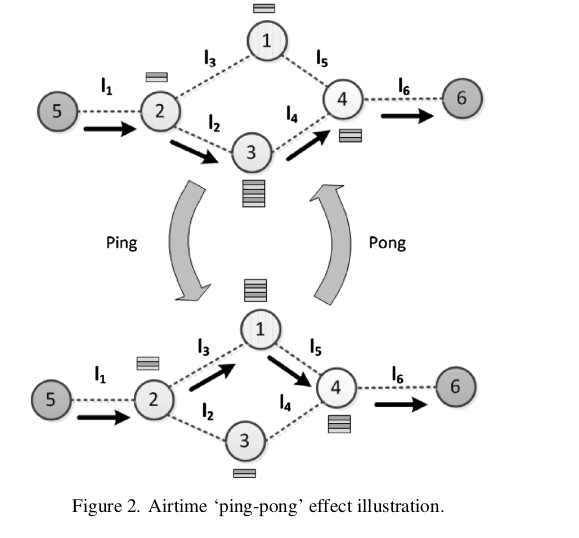
\includegraphics[width=.7\textwidth]{resources/img/chap5/message_exchange}
%					\caption{Message exchange for mesh network advertisement}
%					\label{img:message_exchange}
%				\end{figure}
	
			\subsubsection{Main loop}\label{subsec:loop}
	
				After the code in Figure~\ref{code:mesh_init_2} is executed, the code contains an infinite \texttt{while True} loop.
				Unlike the Arduino, which has the \texttt{loop()} function that runs infinitely unless ordered differently, Pycom devices only execute the contents of \texttt{main.py} once. 
				That is why this infinite loop is needed.
				
				In the FSA in Figure~\ref{fsa:main}, state $ m_{4} $ coincides with this loop.
				It is marked as an accepting state since the program might finish due to possible Exceptions.
				Such Exceptions are part of the ones described later in Section~\ref{sec:software_improvements}.
				
				At each start of the loop, \texttt{LORA\_ANTENNA\_LOCK} is acquired, thus allowing the node to send and receive data.
				This infinite loop can be divided in three parts, which are respectively states $ m_4 $, $ m_5 $ and $ m_6 $ in Figure~\ref{fsa:main}:
				% TODO COMPLETE
				\begin{itemize}
					\item $ m_4 $, listen and for incoming messages and send responses:
					\item $ m_5 $, connection with MegaSense and data gathering:
					\item $ m_6 $, broadcasting mesh advertisement:
						\begin{figure}[H]
							\begin{lstlisting}
node.broadcastMeshAdvertisement(mesh.MESH_ID)
							\end{lstlisting}
							\caption{Code for mesh advertisement in \texttt{main.py} loop}
							\label{code:mesh_advertisement_main}
						\end{figure}
					
						\begin{figure}
							\begin{lstlisting}
def broadcastMeshAdvertisement(self, mesh_id):
  msg = self.MESH_ADVERTISE_PREAMBLE.decode() + 
    "=" + mesh_id.decode() + "." + self.LORA_MAC.decode()
  self.broadcast(msg)
							\end{lstlisting}
							\caption{Code for broadcasting advertisement messages in mesh library}
							\label{code:mesh_advertisement_library}
						\end{figure}
				\end{itemize}	
			
			\subsubsection{Message forwarding}
			
				\textbf{\textcolor{red}{\hl{// To be completed}}}
			
			\subsubsection{MegaSense communication}
			
				If the boolean variable \texttt{MEGASENSE\_CONNECT} in the configuration file is set to \texttt{True}, then at the beginning of \texttt{main()} a \texttt{MegaSense} object is created.
				Such object is implemented in the \texttt{megasense.py} file, a library that contains the functions used to interact with the device.
				
				The architecture of Open LoRa Mesh implies that each node of the network communicates with a MegaSense device via BLE.
				Thus, the configuration file of each node contains \texttt{MEGASENSE\_ADDR} variable, a string with the MAC address of a specific MegaSense.
				If such sensor is in reach, then the node will connect to it and interact, gathering data about air quality in its surroundings.
				Such interaction is done via the functions in the MegaSense class, described in Section~\ref{subsec:megasense_lib}.
				
		\subsection{Mesh library}\label{subsec:mesh_library}
		
				\textbf{\textcolor{red}{\hl{// To be completed}}}
%			\subsection{Node initialization}
%				\begin{figure}
%					\begin{lstlisting}
%def __init__(self) -> None:
%  self.LORA_NETWORK = LoRa(mode=LoRa.LORA, region=LoRa.EU868)
%  self.LORA_SOCKET = socket.socket(socket.AF_LORA, socket.SOCK_RAW)
%  self.LORA_MAC = binascii.hexlify(LoRa().mac())[8:]
%  self.NODE_ID = 0x01
%					\end{lstlisting}
%					\label{code:node_initialization}
%					\caption{Code for node initialization in mesh library}
%				\end{figure}
		
%			\subsubsection{Routing table}\label{subsec:routing_table}
		
%		\subsection{LoRaCTP forwarding}\label{subsec:loractp_mesh}
		
			% spiegare come si modifica loractp
		
%		\subsection{Supported messages}
		
%	\section{LoRa addressing scheme}\label{subsec:lora_addressing}
		
		% Hardware Addressing Schemes
		
		
		%calcolare transmission times
		
%	\section{Other files}
%	
%		Figure~\ref{img:files} shows a list of all files that contribute to this project.
%		
%		\begin{figure}[h]
%			\centering
%			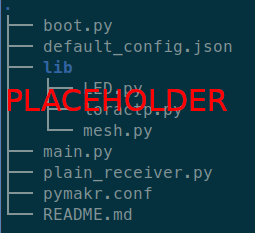
\includegraphics[width=.5\textwidth]{resources/img/chap5/tree_files}
%			\caption{List of files that compose the Open LoRa Mesh project}
%			\label{img:files}
%		\end{figure}
%	
%		\texttt{LED.py} is an LED library that allows the definition of threads in which LED functions are controlled.
%		These are used in the software and have not been explained in the previous sections since their use is secondary compared to the other functions.
%		% TODO CAMBIARE SE NECESSARIO
%		\texttt{README.md} and \texttt{banner.png} files are used in the GitHub repository and not essential to the usability of this project.

		\subsection{MegaSense library}\label{subsec:megasense_lib}
		
	\section{Microcontroller sleep cycle}\label{sec:sleep}
	
		Most IoT devices that compose LPWANs have three main modes, or profiles: \textit{sense}, \textit{connect} and \textit{sleep}.
		Sense and connect refer respectively to gathering data from the sensors and sending it into the network, while sleep refers to a sleep-mode energy consumption where most processes in the device are halted, and some circuits may be powered down.
		It can be considered a design trade-off between functionality, size, and battery lifetime.
		
		This energy consumption profile is important because it helps maximizing the battery life, which currently is one of the most considerable bottlenecks in IoT low-power devices, as explained in Section~\ref{sec:trends}.
		
		However, in the implementation of the Open LoRa Mesh, nodes do not have such functionality implemented, since might it be the cause for network disruptions.
		
		For example, if a new node might want to join a network, but the nearest physical node is in sleep mode, there would be no possibility for the new node to request data about the network, thus wasting time and resources while waiting to the other node to come back online.
		
		Such mode could be implemented but would require an careful analysis on the evolution of the network in time, also would require a network made entirely, or mostly of static nodes.
		This thought is reviewed again in Section~\ref{sec:software_improvements}.
			
	\section{Use cases}
		
		Each network topology is better suited for particular scenarios, and it is not possible to have a ``\textit{one size fits all}'' network.
		Which is why the final section of this chapter explains where Open LoRa Mesh is better suited and where it will not perform as well.
		
		\subsection{Mobile network}
		
			Mobile networks, such as bike sharing and other shared transportation environment, require high speed for adjusting. 
			These are dynamic environments where speed is important, especially for messages exchanged in the control plane, as explained for VANETs in Section~\ref{sec:overview_wms}.
			
			Open LoRa Mesh would not be well suited for such type of networks, this is because the ``\textit{raw maximum data rate of 27 kbps}'' \cite{8030482} and, when moving at high speed, devices can become very sensitive to Doppler effect \cite{s21124049}.
		
		\subsection{Fixed network}\label{sec:fixed_network}
		
			This is the type of network Open LoRa Mesh is better suited in.
			Although MegaSense works with mobile sensors, Open LoRa Mesh would allow it to work with monitoring sensors spread in a defined area.
			This could either be inside or outside a a building.
			
			Such type of network works best since it is mostly static and connections are rarely broken, thus data that needs to be sent in the control plane does not exceed the one sent in the data plane, as it can happen in the previous scenario.
		
		\subsection{Hybrid network}
		
			Such scenario includes, for example, the integration of mobile sensors given to users with a network of fixed sensors in an area.
			In this case, the usability of Open LoRa Mesh depends on the number of mobile devices that need connectivity and how many times they connect and disconnect.
			 	% Proposed solution
 	%!TEX root = ../thesis.tex

\begin{savequote}[60mm]
	There's no reason to have a plan B\\
	because it distracts from plan A.
	\qauthor{Will Smith}
\end{savequote}

\chapter{Experimental results}\label{chapter:results}
	
	This chapter expands the previous one by verifying the usability of Open LoRa Mesh.
	Particularly, it describes four experiments in which Open LoRa Mesh has been set up and tested, in order to record its rough performances.The following sections describe such experiments done with the available hardware in two particular locations: inside a building and in an open field.
	
	The first location is \textit{Archimedes Tower} \footnote{ For simplicity, pictures representing this location are taken from a publicly available online 3D model\newline (\url{https://3dwarehouse.sketchup.com/model/a4d327dd45162ee0557d96e459f19076/})} (\textit{Torre Archimede} in Italian), the building which houses the department of mathematics and computer science at the University of Padova, while the second place is the \textit{Mazzini Square} \footnote{ Images of this location in this thesis are taken from Google Maps and OpenStreetMap} (\textit{Piazza Mazzini} in Italian) in Monselice, a city in the south of Padova.
	
	These places have been chosen especially for their opposite characteristics: Archimedes Tower, in Figure~\ref{img:archimede_1}, is a 31m tall building which develops on seven levels above the ground and three underground levels\footnote{ \url{https://phaidra.cab.unipd.it/view/o:10783}}, while Mazzini Square, in Figure~\ref{img:pzza_mazzini_1}, is an open space that allows an unobstructed view between nodes.
	
	An important remark that has to be done before describing these experiments is that they are not exhaustive.
	When thinking about the amount of possibilities in which nodes can be arranged, it is certain that more tests could have been executed.
	Such kind of system testing has to take in consideration also the surroundings of devices, since they communicate wirelessly.
	
	\begin{minipage}{0.5\textwidth}%
		\begin{figure}[H]
			\centering
			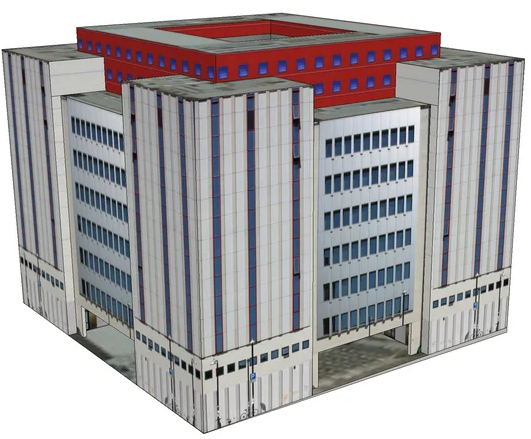
\includegraphics[width=\textwidth]{resources/img/chap5/archimede_1}
			\caption{3D model of Archimedes Tower}
			\label{img:archimede_1}
		\end{figure}
	\end{minipage}%
	\hfill%
	\begin{minipage}{0.5\textwidth}\raggedright
		\begin{figure}[H]
			\centering
			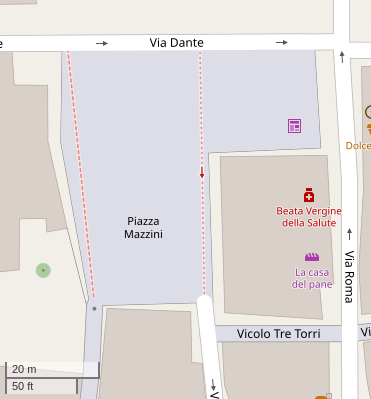
\includegraphics[width=.8\textwidth]{resources/img/chap5/pzza_mazzini_1}
			\caption{View from above of Mazzini Square}
			\label{img:pzza_mazzini_1}
		\end{figure}
	\end{minipage}%
	
	\section{Board placement}
	
		For these experiments, all four boards have been used to test the functionalities of the network.
		Placement of the boards is represented for both locations, respectively in Figure~\ref{img:archimede_2} for Archimedes Tower and in Figure~\ref{img:pzza_mazzini_2} for Mazzini Square.
		
		\begin{figure}[h]
			\centering
			\includegraphics[width=.6\textwidth]{resources/img/chap5/archimede_2}
			\caption{Placement of boards in Archimedes Tower}
			\label{img:archimede_2}
		\end{figure}
	
		Regarding Archimedes Tower, boards have been placed so that board \textbf{\textit{A}} is on the 6$^{th}$ floor, \textbf{\textit{B}} is on the 4$^{th}$ floor, \textbf{\textit{C}} is on the 2$^{nd}$ floor, \textbf{\textit{D}} is on the first underground level.
		All boards have been placed with the antenna facing the internal courtyard of the building.
		
		For Mazzini Square, on the other hand, boards have been placed so that they are directly visible to each other, almost one for each corner of the square.
		
		\begin{figure}[h]
			\centering
			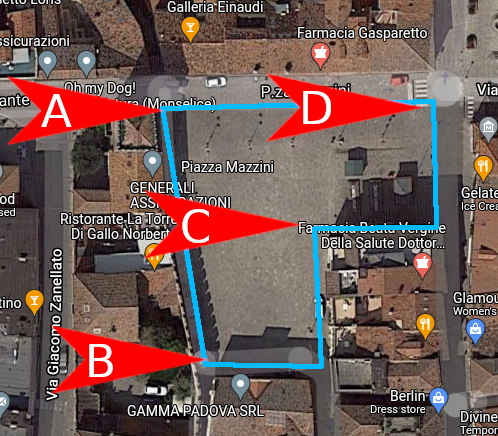
\includegraphics[width=.75\textwidth]{resources/img/chap5/pzza_mazzini_3}
			\caption{Placement of boards in Mazzini Square}
			\label{img:pzza_mazzini_2}
		\end{figure}
	
		These placements have been made so that boards do not have direct obstructions that can block the signal in between them.
		Such placement can be considered ideal because nodes are not far from one another, and their signal does not lose much power.

		In both scenarios boards have been tested as if they were part of a network of fixed devices, which, as explained in Section~\ref{sec:fixed_network}, is the best case scenario for Open LoRa Mesh.
	
	\section{Experiments}
		
		Following there are the four experiments done to test the usability of the network: \textit{message range}, \textit{mesh creation}, \textit{node addition} and \textit{node removal}.
		These sections contain a description on how these experiments have been executed and the results achieved.
		
		\subsection{Message range}
		
			This first experiment is intended to understand nodes' range and how they can be placed in order to achieve a strongly connected network.
			
			In the case of Archimedes Tower, this test has shown the weakness of LoRa when devices are placed inside a building.
			Considering the placement of nodes as represented in Figure~\ref{img:archimede_2}, various cases have been examined.
			
			To test the transmission range of the nodes in the worst-case scenario, at first device \textbf{\textit{D}} has been booted on the library's floor.
			After booting up, the device listens for around 180 seconds for any mesh advertisement messages, as explained in Section~\ref{subsec:initialization}, but since there are no other nodes on it will create a new mesh with the specified identifier.
			Subsequently, device \textbf{\textit{A}} was the second one started, but, due to the number of concrete layers in between these devices, not all packets were correctly exchanged in between these two nodes.
			This has caused device \textbf{\textit{A}} not being able to exchange data with node \textbf{\textit{D}} and to be shut down so that a better placed node could be booted up.
			Node \textbf{\textit{B}}, placed on the 4$^{th}$ floor, showed better results when exchanging mesh data, although some messages were still lost when communicating with node \textbf{\textit{D}}.
			
			The best placement of nodes in Archimedes Tower is thus represented by the placement in Figure~\ref{img:archimede_1}.
			Nodes have shown a strong connection when placed roughly two levels apart and booted up in order, allowing the mesh to be created without any packet loss.
			FiPys have been booted in alphabetical order and two minutes apart from each other, so the first one would have time to generate the mesh, and the others would be able to join it.
			The creation of a mesh and the addition of a node are further described in  Section~\ref{subsec:node_addition}.
			
			Contrasting with the thick walls of Archimedes Tower, Piazza Mazzini is an open space where no obstructions are present.
			In this scenario, whatever is the order in which devices are booted, all of them have a clear line of sight with one another.
			This resulted in a network where nodes have a strong connection with one another and do not require any particular though on antenna placement, as long as these are facing the inside of the square.
			
			Such differences in results are the reason why places so divergent have been chosen for testing the mesh.
			They show how space around nodes influences the network and that it is important to study an ideal placement that can allow the mesh to function correctly and with as little packet loss as possible.
			A scenario similar to Mazzini Square can be an orchard, where each node is strategically placed to monitor part of the field and relates data on air measurements, since for every FiPy there should be a MegaSense paired.
			
		\subsection{Mesh creation and node addition}\label{subsec:node_addition}
		
			As long as nodes are in reach of one another, the creation of the mesh and the addition of a node are quite straightforward.
			When the first node boots, it needs around 180 seconds to go beyond the initial listening phase, since there are node preexisting networks.
			
			In Archimedes Tower's case, by booting devices in alphabetical order, or reverse, the mesh would create without any issues since, as stated in the previous section, FiPy's range would not be affected as much when devices are separated by two floors. 
			
			Creating a mesh in Mazzini Square produced similar results compared to Archimedes Tower.
			Since here devices' range is not obstructed, only the time in mesh creation is considered.
			
			In both scenarios, the minimum time to correctly initiate the mesh network has proven to be around 5 minutes, considering the first node needs 3 of them to create the mesh and then booting the others 30 seconds apart after.
			
			Node addition can be tested while testing the correct creation of the mesh network.
			Booting up node by node, it can be seen that the routing table correctly creates for each device.
			Environment, as previously mentioned, has to be taken in consideration.
			This is because a strong reception is required in between nodes.
			
		\subsection{Node removal}
		
			This experiment tests the robustness of the network when a node is abruptly removed.
			Results of such test diverge, according to the environment.
			
			In Archimedes Tower, the removal of either of the external nodes results in a mesh that keeps functioning and allows messages to be exchange in between the remaining devices.
			The mesh heals by recreating the routing table and removing the device that was suddenly shut down.
			
			If the device shut down is one in the middle of the building, the one on floor $4$ for example, the mesh will have a harder time to recreate, given the previously talked about connectivity problem of nodes in such environment.
			
			In Mazzini Square the removal of a node resembles the first case described for Archimedes Tower.
			Since devices have a clear line of sight, the mesh does not have any problems to heal.
	
	\section{About the results}
		
		In order to achieve an optimal connectivity in Archimedes Tower, nodes would need to be placed near the window on each of the aforementioned floors ($-1$, $2$, $4$, $6$).
		Placing them near the window, either facing externally or on the internal courtyard, would allow them to have a clear visual: a stronger connection could then be achieved in between nodes \textbf{\textit{A}} and \textbf{\textit{D}}.
		
		The same approach applies to Mazzini Square, where devices have been placed on almost each corner of the square, thus being outside.
		If they where to be placed inside of the buildings facing the square, antennas would need to be near windows or outside.
		
		Placing the devices inside of Archimedes Tower means collecting air quality information in the building, possibly in the staircase, or in classrooms or offices.
		This allows the MegaSense device, or other sensors that could attach to the network, to record this data and create o model of air quality inside the building.
		
		On the other hand, placing the FiPys in Mazzini Square would allow MegaSense devices to collect data on air quality in regarding a large open area.
		If thoroughly recorded, data from this area could be an interesting start for a research on pollutants of 	cement plants, given that Monselice has two of them.
		
		By booting multiple nodes at the once, the random time added to the initial 180 seconds in which each node is listening, prevents devices to create separate multiple meshes.
	
	\section{Other possible experiments}
	
		Nothing is ever perfect, thus it is important to keep improving and test the work done.
		The aforementioned tests are not conclusive to declare Open LoRa Mesh ready for a ``\textit{production environment}'', where nodes can rely on the structure of the network to send their data.
		These tests only show that Open LoRa Mesh is a valid starting point to build upon and provide an interesting possibility in using LoRa as a transmission method.
		Also, as said earlier, the placement of nodes in the test can be considered ideal when thinking about signal strength and reach of LoRa antennas.
		
		A consideration on how other transmission methods would work compared to LoRa is talked about in Section~\ref{sec:other_transmission_methods}. 	% Results and experimentation
	%!TEX root = ../thesis.tex

\begin{savequote}[70mm]
	Be fearful when others are greedy,\\
	and greedy when others are fearful.
	\qauthor{Warren Buffet}
\end{savequote}

\chapter{Conclusions}\label{chapter:conclusions}

	Mesh networks are ``\textit{decentralized, easy to deploy, and characterized by dynamic self-organization, self-configuration, and self-healing properties}'' \cite{Sampaio-2015}.
	Such properties enable fast deployment, low installation cost, and reliable communication.
	
	This thesis describes an implementation of a mesh network solution for IoT devices, particularly for an air quality sensing device: MegaSense, described in Section~\ref{subsec:megasense}.
	
%	This project represents
%	
%	It has been implemented on pycom hardware, the software is available on github in 
	
	Besides summarizing the previously discussed arguments, this chapter contains some personal considerations by the author.

	\section{Contributions}
	
		\textbf{\textcolor{red}{\hl{// To be completed}}}

	\section{Future work}
		
		\textbf{\textcolor{red}{\hl{// To be completed}}}
	
		\subsection{Hardware improvements}
			
%			Note from the author, it must be taken in consideration that the device can run hot, an application of the device such as on a bike that is parked out in the sun may overheat the device.
%			On pycom's documentation it is written that the fipy can support temperatures up to x
%			Thus an interesting improvement could be to add a heatsink in order to lower the temperatures and improve the lifespan of the device
		
			\textbf{\textcolor{red}{\hl{// To be completed}}}

		\subsection{Software improvements}\label{sec:software_improvements}
		
			\textbf{\textcolor{red}{\hl{// To be completed}}}
		
%			Better logging 
%			
%			improvement on routing table and algorithm used for message forwarding 

%			Aggiungere altre modalità oltre a quella di plain listener e del main, ad esempio relay station per fare forwarding dei messaggi

			Another factor that would improve the performance of each node on the network is the implementation of a sleep mode, Section~\ref{sec:sleep}.
			This would allow each node to have a longer battery life and only activate when necessary.
			Although adding such mode requires more data and in depth testing, it is not an impossible upgrade.

	\section{Personal considerations}
	
		This final section of the thesis contains some personal considerations from the author regarding the work with Pycom boards and mesh networks.
	
		\subsection{About the Pycom boards}\label{sec:working_with_pycom}
		
			Compared to working with other boards, such as the Arduino, Pycom boards are more complete, since they offer better specifications, for both computing power and memory, connectivity and support.			
			For prototyping, Arduino boards offer very good opportunities and have been on the market for a longer time, allowing consumers to get acquainted and know the brand.
			% https://patentlyo.com/patent/2011/01/tracing-the-quote-everything-that-can-be-invented-has-been-invented.html
			Sometimes, working with Arduino feels like ``\textit{everything that can be invented has been invented}'', as said by Charles H. Duell, since there is so many people who have made all kind of projects and are sharing them online.
			
			The FiPy, on the other hand, offers more connectivity and more power, at the expense of the open source advantages of most of its competitors.
			As explained in Section~\ref{sec:pycom}, besides keeping the blueprints of their boards private, Pycom also has a proprietary firmware on their boards, which sometimes gets in the way of developers that require to fully use the hardware capabilities.
			This also reflects on the software, where some functionalities that are functioning on other boards are not implemented in Pycom's firmware for their devices.
			Nonetheless, the official forum\footnote{ \url{https://forum.pycom.io/}} available for Pycom's boards is full of useful comments and the users are fairly active.
			
			An example where the FiPy would offer a great improvement over an Arduino board would be this smart home application\footnote{ \url{www.instructables.com/Smart-Home-With-Arduino-Ethernet-Shield-and-Teledu}}.
			Such project contains an Arduino Mega board with various sensors and relays, all connected via a specifically build website, with the use of a third-party API handler for the Arduino.
			The Arduino connects to the Internet via an Ethernet shield, thus sends data by cable.
			A FiPy would allow a smaller footprint and no need for a shield, besides avoiding the use of a third-party API handler.
					
			In my personal opinion, these boards are quite powerful and resilient for research purposes.
			They can be used as multiple testbenches for different projects, but might result excessive if their powerful specifications are not necessary.
			
		\subsection{About mesh networking}\label{sec:mesh_considerations}
			
			As said in Chapter~\ref{chapter:technologies}, each network topology is better suited for particular scenarios.
			It is not possible to have a ``\textit{one size fits all}'' network for all possible applications that need to exchange data.
			As for all questions in computer science, the answer to the question where a mesh network is useful is ``\textit{it depends}''.
			
			Mesh networking is a very interesting network topology which, compared to all the others in Figure~\ref{img:network_topologies}, has still a lot of research possibilities.
			In conjunction with AI and machine learning, it is possible to achieve an optimal level of connectivity in such networks.
			The bottlenecks would then be represented by the computing power in the nodes, and in the algorithm used in case one of the nodes fail, or new nodes are added into the network.

			Scalability of such networks, as spoken about in Section~\ref{sec:scalability}, is a very interesting research scenario since it is one of the major deciding elements for any new networking technology to be accepted.
			Factors such as multi-hopping, protocol overhead, and wireless interference limit the scalability of such networks.
			Mesh networks will be more and more common, but I believe they will be used in conjunctions with other topologies: for example a local mesh network that allows communication between sensors in a house and a gateway node interacts with other networks in a different topology.
			
			Security is another important factor when considering in mesh networking.
			Since each node receives and analyzes packages, there is no totally effective solution for a secure network.
			Adding security features such as encryption/decryption algorithms and other checks, would result in a big overhead on small IoT devices.
			Also, like other radio technologies, anyone can read messages, encrypted or not, ``\textit{flying}'' through the air. 	% Conclusions
	
	% %!TEX root = ../thesis.tex

\renewcommand\thechapter{A}
\chapter{User Manual}\label{ch:AppendixA}
	
	
	
% TODO spostare le cose commentate in capitolo 5
%	The author has decided to add this appendix to the thesis as a small documentation on how to interface and program the pycom boards.
%	
%	The main documentation can be found at % https://docs.pycom.io/
%	
%	In particular this appendix contains the instructions on how to program the Fipy and pytrack, which, as described in [reference to section where I described the used hardware], are the components that the author has used in this thesis
%	
%	Online forum 
%	% https://forum.pycom.io/category/24/getting-started
%	
%	Youtube channel
%	% https://www.youtube.com/c/Pycom/videos
%	
%	Github
%	% https://github.com/pycom/pycom-libraries
%	
%	\section{Requirements}
%		
%		\subsection{Hardware}
%		
%			In order to interface and program the FiPy it is important to 
%			
%			insert image of uart device
%			% https://docs.pycom.io/gettingstarted/programming/usbserial/
%			% https://www.circuitbasics.com/basics-uart-communication/
%			
%			alternatively it can be programmed via the pybytes platform
%			% https://pycom.io/new-pymesh-on-pybytes-video-tutorial/
%		
%			How to configure antennas for the 
%			% https://pycom.github.io/pydocs/gettingstarted/connection/fipy.html#third
%		
%		\subsection{Software}
%		
%			note to update firmware
%			% https://pycom.github.io/pydocs/pytrackpysense/installation/firmware.html
%			% https://core-electronics.com.au/videos/pycom-pytrack-and-pysense-how-to-update-firmware
%			
%			% https://cloud.google.com/architecture/tracking-assets-with-iot-devices-pycom-sigfox-gcp
%			
%			
%			clear flash memory
%			% https://forum.pycom.io/topic/2620/error-when-importing-pysense-pytrack/6
%			% https://docs.pycom.io/gettingstarted/programming/safeboot/
%			
%	\section{Programming the FiPy}
%	
%		\subsection{Hello world}
%		
%		
%		\subsection{Where am I?}
%			% https://docs.pycom.io/datasheets/expansionboards/pytrack2/ 
	% %!TEX root = ../thesis.tex

\renewcommand\thechapter{B}
\chapter{Appendix B}\label{ch:AppendixB}

	\lipsum[1-2] 
	
	\addcontentsline{toc}{chapter}{Acknowledgments}
	\acknowledgments
	
	\cleardoublepage
	\phantomsection
	
	\addcontentsline{toc}{chapter}{References}
	\bibliography{references}
	
	\cleardoublepage
	\phantomsection
	
%	\addcontentsline{toc}{chapter}{Glossary}
%	\printglossary

	\backmatter

\end{document}